% 第十一届湖南省研究生数学建模竞赛 B 题论文
% 版式对齐：competition_question/（必读）第十一届湖南省研究生数学建模竞赛论文格式规范.docx
% 匿名：无队号、单位、姓名；页眉空白（规范禁止页眉出现队号）；页脚中部页码自 1
% 编译：bash compile.sh  或  xelatex main.tex （两次）
\documentclass[UTF8,a4paper,zihao=-4,fontset=fandol]{ctexart}

% 页边距取规范 Word 的上下 2.54cm，左右按惯例不少于 2.5cm
\usepackage[a4paper,top=2.54cm,bottom=2.54cm,left=2.54cm,right=2.54cm]{geometry}
\usepackage{amsmath,amssymb,bm}
\usepackage{booktabs,tabularx,multirow,makecell}
\usepackage{graphicx}
\usepackage{caption}
\usepackage{setspace}
\usepackage{enumitem}
\usepackage{xcolor}
\usepackage{fancyhdr}
\usepackage[hidelinks]{hyperref}
\usepackage{listings}

% 正文英文：Times 同类（本机无 Times New Roman 时用 TeX Gyre Termes）
\setmainfont{TeX Gyre Termes}[
  Extension      = .otf,
  UprightFont    = texgyretermes-regular,
  BoldFont       = texgyretermes-bold,
  ItalicFont     = texgyretermes-italic,
  BoldItalicFont = texgyretermes-bolditalic,
  Path           = /usr/share/texmf/fonts/opentype/public/tex-gyre/,
  Ligatures      = TeX,
]

\hypersetup{pdftitle={考虑送端碳排不确定性的区域电网鲁棒碳流追踪与低碳调度},pdfauthor={},pdfcreator={}}

\graphicspath{{../src/outputs/q1/}{../src/outputs/q2/}{../src/outputs/q3/}{../src/outputs/q4/}{../src/outputs/deepen/}}

% 题目三号黑体居中；一级小三黑左齐；二级四号黑左齐；三级小四黑左齐（均加粗、不居中）
\ctexset{
  section/format = \heiti\zihao{-3}\bfseries\raggedright,
  section/beforeskip = 0.7ex plus .2ex,
  section/afterskip = 0.45ex plus .1ex,
  subsection/format = \heiti\zihao{4}\bfseries\raggedright,
  subsection/beforeskip = 0.55ex plus .2ex,
  subsection/afterskip = 0.35ex plus .1ex,
  subsubsection/format = \heiti\zihao{-4}\bfseries\raggedright,
  subsubsection/beforeskip = 0.4ex plus .1ex,
  subsubsection/afterskip = 0.25ex,
}
% 正文小四宋体、单倍行距、段前段后 0.25 行、首行缩进 2 字符
\setstretch{1.0}
\setlength{\parskip}{0.25\baselineskip}
\setlength{\parindent}{2em}
\setlist{nosep,leftmargin=2em}

% 图注、表头：楷体 11 号
\DeclareCaptionFont{kai11}{\kaishu\fontsize{11pt}{15pt}\selectfont}
\captionsetup{font=kai11,labelsep=quad,skip=4pt}
\captionsetup[table]{position=top,skip=3pt}
\captionsetup[figure]{position=bottom,skip=3pt}

\renewcommand{\thefigure}{\arabic{figure}}
\renewcommand{\thetable}{\arabic{table}}
\renewcommand{\theequation}{\arabic{equation}}

% 页眉空白；页脚中部阿拉伯页码
\pagestyle{fancy}
\fancyhf{}
\fancyfoot[C]{\thepage}
\renewcommand{\headrulewidth}{0pt}
\renewcommand{\footrulewidth}{0pt}
\fancypagestyle{plain}{%
  \fancyhf{}%
  \fancyfoot[C]{\thepage}%
  \renewcommand{\headrulewidth}{0pt}%
}

\lstset{
  basicstyle=\ttfamily\zihao{6},
  language=Python,
  breaklines=true,
  columns=fullflexible,
  frame=single,
  rulecolor=\color{black!25},
  aboveskip=4pt,
  belowskip=4pt,
  showstringspaces=false,
  keywordstyle=\bfseries,
}

\begin{document}

% 第 1 页：竞赛名（对齐规范 Word 题头）+ 论文题目 + 摘要 + 关键词
\begin{center}
{\heiti\zihao{-2}\bfseries 第十一届湖南省研究生数学建模竞赛}\\[1.4em]
{\heiti\zihao{3}\bfseries 考虑送端碳排不确定性的区域电网}\\[0.35em]
{\heiti\zihao{3}\bfseries 鲁棒碳流追踪与低碳调度}
\end{center}
\vspace{1.1em}

\noindent{\heiti\zihao{-4}\bfseries 摘\quad 要}\quad
针对某省八区域电网“计量口径不一、碳随电走、五年项目耦合、省外送端碳因子波动”四重困难，本文按“校数—追碳—选项目—防不确定”建立可复现链条。问题一将多源电量校正表述为守恒约束下的加权最小二乘数据调和，等价于面向能量平衡的广义状态估计；识别异常 23 处，调和后 $\chi^2/n=0.2417$，通道 E05 线损由工程值 0.020 修正为 0.0135。问题二在比例共享下逐月求解节点碳势：A4 终端碳强度 0.624\,kgCO$_2$/kWh，A5 仅 0.152；A3 消费责任为生产责任的 5.36 倍，主碳流为 A4$\to$A3（4374\,kt）。生产—消费线性共担在 $\lambda=0.5$ 时与通道碳转移博弈的 Shapley 值（$2^8$ 精确枚举）一致，从而为五五分成提供公理化。问题三以省级碳上限为硬约束、区域预算为软约束建立五年 MILP：无项目基准五年累计越限 567\,kt，贪心可行解投资 976.2 百万元即可贴上限，MILP 主方案投资 985.5 百万元、入选 7 个项目且全部达标；通道升级因官方碳口径不依赖潮流而未入选。问题四将送端因子扰动经 2025 年份额矩阵 $S_{ij}$ 传导：确定性方案在 S3 情景下 2030 年越限 454.5\,kt；静态 $\Gamma$-鲁棒与稳健滚动均可零越限，但实物投资升至 4848.8 百万元（溢价 3863.3）。滚动在“未来年始终按 $\Gamma=1$ 设防”规则下并不自动少投资，其价值是逐年确认决策、剩余期目标由 6130.6 降至 5614.0 百万元。据此建议：考核用五五共担，基准路径用 985.5 百万元方案，日常执行用滚动，压力底线用静态鲁棒。

\vspace{0.6em}
\noindent{\heiti\zihao{-4}\bfseries 关键词：}\ 数据调和；碳排放流；责任共担；项目组合优化；预算鲁棒优化

\newpage

\section{问题重述}

某省一次能源不足，电力消费对省外输入存在刚性依赖。省内八个区域（记为 $A1,\ldots,A8$）产业结构、电源结构与发展阶段分化明显，区域间由 11 条通道互联。电力来源的碳排放强度差异大，区域用电的碳责任不能只按本地发电核算。2026—2030 年将滚动实施工业节能、建筑改造、交通电气化、分布式光伏及通道升级等 35 个候选项目，项目之间存在资源竞争、互斥与协同。与此同时，省外送端电源结构随季节与供需变化，输入电的碳因子并非常数。

附件给出 2025 年分月监测、年度汇总、通道工程参数、排放因子、五年双控约束、项目库以及送端碳因子区间与情景。数据来自不同监测系统，存在缺失、口径差与个别物理上不合理的记录。题面能量平衡为
\begin{equation}
G_{i,t}+I_{i,t}+\sum_{j\neq i}T_{j,i,t}
=D_{i,t}+\sum_{j\neq i}T_{i,j,t}+L_{i,t},
\label{eq:balance}
\end{equation}
其中 $G$ 为本地发电，$I$ 为省外输入，$T$ 为区域间输电，$D$ 为终端用电，$L$ 为损耗；因测量误差，\eqref{eq:balance} 在原始数据上并不成立。电量单位为 GWh，与排放因子（kgCO$_2$/kWh）相乘得碳排放（ktCO$_2$）。

需要依次回答五个问题：（1）识别并校正多源电量，估计通道损耗，评价观测影响度；（2）追踪碳流，给出逐月终端碳强度，并按发电地、用电地及兼顾二者的口径分担责任；（3）在供能与全省碳上限下安排五年项目，使综合成本合理，并检验方案稳定性；（4）评估送端碳因子不确定对问题三方案的冲击，给出仍可满足约束的调整机制并量化抗风险代价；（5）面向选定决策主体撰写约 1000 字咨询报告。附件 6 的题面文字写“突发事件”，Excel 给出的是碳因子上下界与情景 S0—S3，\textbf{本文以 Excel 为准}。

\section{问题分析与技术路线}

四问不是并列的四个模型，而是一条必须守住因果顺序的链条：没有守恒的电量台账，碳势没有物理意义；没有 2025 年区域碳强度，五年碳约束无法落到项目；没有问题三的基准方案，就无法定义“不确定冲击有多大”和“抗风险要多花钱”。

问题一的本质是过程系统中的数据调和：在硬守恒下用加权最小二乘把冗余观测拉回到可行流形，并用标准化残差找粗差。它与电力系统加权最小二乘状态估计同构，区别仅在于状态是区域—月度电量与通道损耗，而不是相角电压。问题二把比例共享从潮流追踪推广到碳：同一节点的出流携带同一碳势，碳量随到达电量走。责任核算需要同时报告生产侧、消费侧，以及把二者连起来的共担规则，并用全省总量守恒做正确性检验。问题三是多年期投资—运行耦合的混合整数规划：省级碳上限硬约束决定“能不能达标”，区域软预算决定“超标罚多少”，项目侧的资源、投资、互斥与协同决定可行集。问题四在预算不确定集上做对等式鲁棒，再用两阶段可调鲁棒区分“此时此地”与“观望”，最后用滚动时域把已观测年份换成真值。

技术路线如图式所示：附件 1/2 $\to$ 问题一调和 $\to$ 附件 3 与碳势方程 $\to$ 问题二责任与份额矩阵 $S_{ij}$ $\to$ 附件 4/5 的五年 MILP $\to$ 附件 6 的情景与 $\Gamma_t$ $\to$ 咨询报告。计算栈为 Python 3、cvxpy/Clarabel（二次规划）、Pyomo/HiGHS（MILP）。全部数字由脚本写入 \texttt{src/outputs/}，正文不手填。

\section{基本假设与符号}

\subsection{基本假设}

\begin{enumerate}[label=\textbf{H\arabic*.}]
\item 校正后的月度电量满足区域能量平衡；通道损耗落在线路上，入流按受端计量、出流按送端计量。
\item 区内输配损耗无直接关口，采用“终端用电 $\times 5\%$”作为可松弛先验，不把损耗钉死在 5\%。
\item 碳流采用比例共享与送端承担线损碳的主口径；节点碳势由入流碳量守恒唯一确定。
\item 2026—2030 年区域终端碳强度沿用 2025 年追踪结果，再用附件给出的 $\kappa_y$ 做全省强度调整；官方碳核算不显式依赖区域间潮流。
\item 问题四把 2025 年“省外输入分接入区”份额矩阵 $S_{ij}$ 冻结到 2030 年。这是强假设，后文给出定量局限。
\item 送端不确定只用附件 6 的因子区间与情景，不另造突发事件时间线。
\item 项目效益自开工年加建设周期起生效；已开工规模在滚动中不可逆。
\item 主方案综合成本不折现，与附件年度投资上限同口径；8\% 折现仅作敏感性。
\end{enumerate}

\subsection{主要符号}

\begin{table}[htbp]
\centering
\caption{主要符号}
\label{tab:symbol}
\begin{tabular}{llp{7.6cm}}
\toprule
符号 & 单位 & 含义 \\
\midrule
$i,j$ & --- & 区域，$i,j\in\{A1,\ldots,A8\}$ \\
$t,y$ & --- & 月份（2025）或规划年（2026—2030） \\
$x_k,\hat x_k,\sigma_k$ & GWh & 观测、校正值、不确定度 \\
$\eta_e$ & --- & 通道 $e$ 损耗率 \\
$\rho_{i,t}$ & kgCO$_2$/kWh & 节点碳势（终端用电碳强度） \\
$P^+_i,C^+_i$ & ktCO$_2$ & 扩展生产责任、全口径消费责任 \\
$F_{j\to i}$ & ktCO$_2$ & 通道 $j\to i$ 到达电量携带的碳 \\
$S_{ij}$ & --- & 区域 $i$ 消费中来自接入区 $j$ 省外输入的份额 \\
$E_{i,y}$ & ktCO$_2$ & 规划年消费侧碳排放 \\
$\overline E_y$ & ktCO$_2$ & 全省消费侧碳上限 \\
$B_{i,y}$ & ktCO$_2$ & 区域软预算 \\
$w_y$ & --- & 预算惯性权重（0.85$\to$0.65） \\
$\xi_{j,y}$ & --- & 送端因子相对基准的乘数 \\
$\Gamma_y$ & --- & 年份 $y$ 的不确定预算 \\
$\tau$ & --- & $\Gamma$ 缩放（price of robustness） \\
\bottomrule
\end{tabular}
\end{table}

\section{问题一：多源电量一致性校正}

\subsection{异常识别}

在求解调和模型之前，先做不依赖优化器的结构性校验：分部门用电是否加总为终端用电、月度累加是否与年度汇总一致、通道隐含损耗是否偏离工程值、是否出现受端大于送端、容量是否越限，以及把缺失的区内损耗按 5\% 终端用电代入后能量平衡的标准化残差。以 $|z|>3$ 为粗差阈值。共得到 23 条记录。最严重的是 2025-09 区域 A2 的平衡残差 $z=32.5$（与该月工业用电、终端合计同时缺失一致）；通道 E03 在 8 月隐含损耗率 0.175，远高于工程值 0.025；E10 年度汇总受端 1563.8\,GWh 大于送端 1559.6\,GWh。月度与年度两套系统在 A2 工业用电上偏差 8.71\%。四个月度空值（A7 风电、A4 水电、A2 工业与终端合计）在模型中作为自由变量。

\subsection{守恒约束下的加权最小二乘}

记全部待校正量为 $\hat{\boldsymbol x}$（分源发电、省外输入、分部门用电、通道送/受端电量）及区内损耗 $\boldsymbol L$ 与通道损耗率 $\boldsymbol\eta$。目标取加权平方和\cite{Crowe1996data,Narasimhan1999data}
\begin{equation}
\min_{\hat{\boldsymbol x},\boldsymbol L,\boldsymbol\eta}
\sum_{k\in\mathcal O}
\left(\frac{\hat x_k-x_k}{\sigma_k}\right)^2
+\sum_{i,t}\left(\frac{L_{i,t}-0.05\,D_{i,t}}{0.5\times 0.05\,D_{i,t}}\right)^2
+\sum_e R_\eta(\eta_e;\eta_e^{\mathrm{eng}}),
\label{eq:wls}
\end{equation}
其中 $\mathcal O$ 为非缺失观测，$\sigma_k=\max(\mathrm{rel}_k\cdot|x_k|,\underline\sigma_k)$。相对不确定度取发电/输入/分项用电 2\%、终端合计与年度汇总 1.5\%、通道计量 2.5\%。约束为：每个区域—月份的能量平衡\eqref{eq:balance}（入流用受端电量、出流用送端电量）；$0\le$ 受端 $\le$ 送端 $\le$ 月度容量；工程记录为零的通道强制零流；损耗率由送受端电量定义并与工程值正则化。该问题是带线性守恒的凸二次规划，即广义 WLS 状态估计\cite{Schweppe1970power,Abur2004power}。区内损耗作为非负自由变量进入平衡，5\% 先验只起收缩作用。多源电量在守恒约束下做排放追踪的实证同构见文献\cite{deChalendar2021physics}。

标准化残差 $|(\hat x-x)/\sigma|>3$ 用于事后核对粗差处理是否过度扭曲观测\cite{Abur2004power}。通道损耗率在“固定 $\eta$ 调和电量—由电量更新 $\eta$”之间迭代两次。观测影响度采用留一扰动：把关键年度或月度观测上调 5\% 后重解，以全省区域用电变化与线损变化的加权幅度排序。

\subsection{校正结果}

调和收敛，目标函数 307.9，观测项 1274，$\chi^2/n=0.2417$，显著小于 1，说明在所取 $\sigma$ 下模型没有系统性欠拟合。平衡残差最大 $5.8\times 10^{-13}$\,GWh，硬约束在数值上成立。四处缺失的插补为 47.89、64.67、493.56、881.25\,GWh（依次为 A7 风电、A4 水电、A2 工业、A2 终端）。全省调和后区内损耗率 1.78\%，并没有被先验钉在 5\%。通道损耗总体贴近工程记录，但 E05 由 0.020 降为 0.0135，E03 由原始隐含 0.043 拉回到 0.027 附近。影响度最高的三项是 E10 年度送端汇总、A5 年度终端用电、A4 年度省外输入——它们处于“两套系统对账 + 枢纽关口”的位置，建议优先做口径对齐。通道工程线损与调和估计的对照见图\ref{fig:eta}。

\begin{figure}[htbp]
\centering
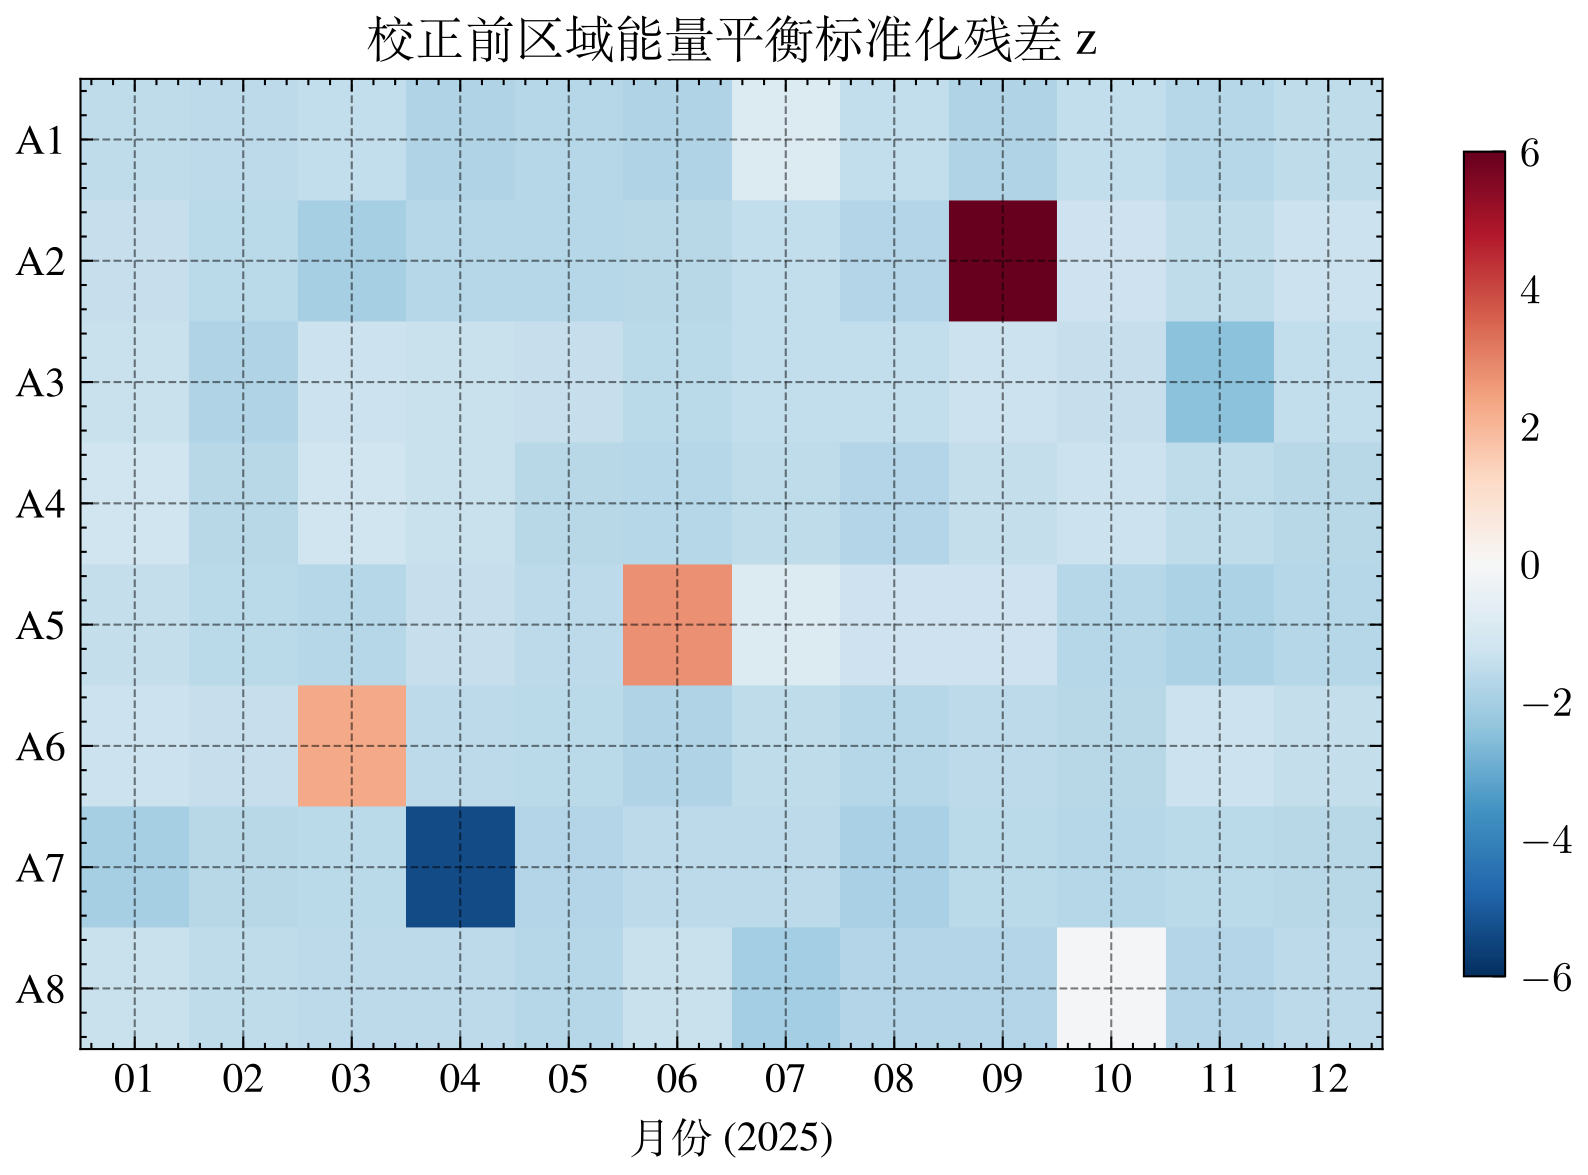
\includegraphics[width=0.92\textwidth]{fig_q1_raw_residual_heatmap.png}
\caption{校正前各区域—月份能量平衡标准化残差。颜色为 $z_{i,t}=r_{i,t}/\sigma_{i,t}$；$|z|>3$ 对应 A2 九月等粗差。}
\label{fig:q1res}
\end{figure}

\begin{figure}[htbp]
\centering
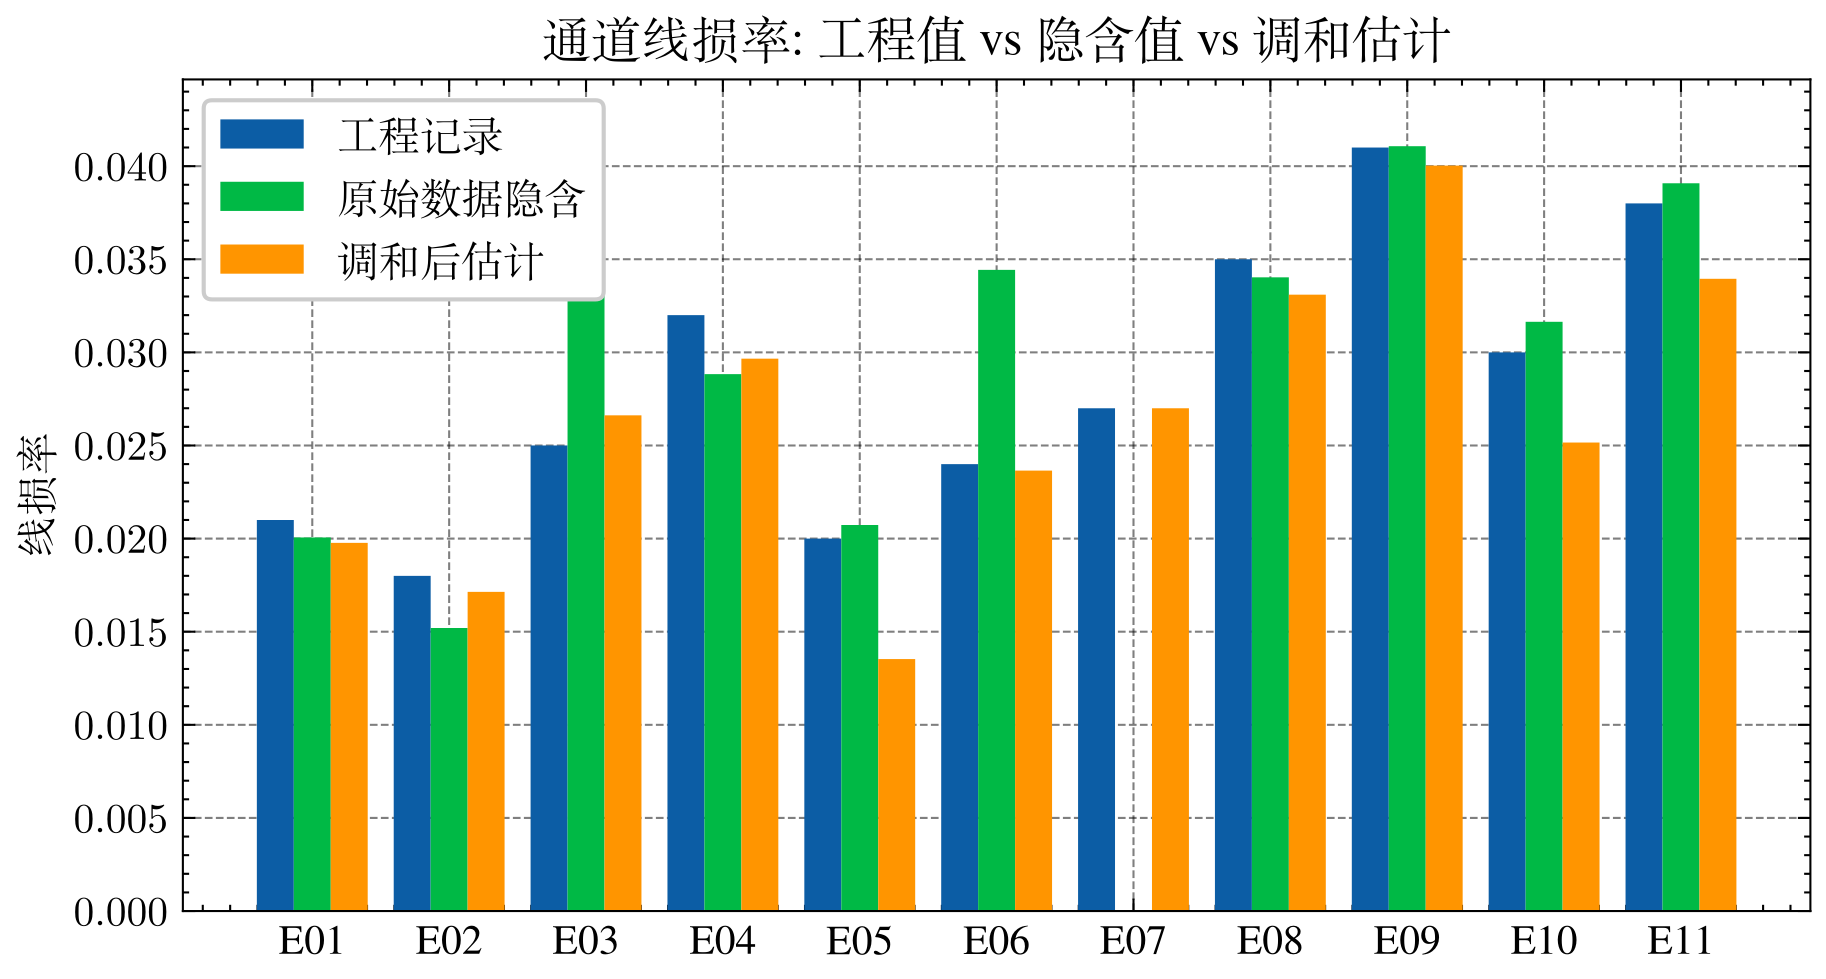
\includegraphics[width=0.88\textwidth]{fig_q1_eta_compare.png}
\caption{通道工程线损率与调和后估计。E05 由 0.020 降至 0.0135；E03 由原始隐含偏高被拉回工程值附近。}
\label{fig:eta}
\end{figure}

\begin{table}[htbp]
\centering
\caption{区内损耗先验与量测 $\sigma$ 的敏感性}
\label{tab:q1sens}
\begin{tabular}{lccc}
\toprule
设定 & $\chi^2/n$ & 区内损耗率 & E05 线损 \\
\midrule
损耗先验 3\% & 0.1879 & 1.756\% & 0.01294 \\
损耗先验 5\%（主方案） & 0.2417 & 1.775\% & 0.01353 \\
损耗先验 8\% & 0.2778 & 1.551\% & 0.01495 \\
相对不确定度 $\times 0.5$ & 0.3727 & 0.880\% & 0.01354 \\
相对不确定度 $\times 2$ & 0.1245 & 3.250\% & 0.01609 \\
\bottomrule
\end{tabular}
\end{table}

表\ref{tab:q1sens}表明：先验从 3\% 调到 8\%，E05 仍明显低于工程值 0.020；把 $\sigma$ 整体缩小或放大一倍，E05 在 0.0135—0.0161 之间，不改变“工程记录偏高”的方向。5\% 与基准 $\sigma$ 是建模选择，不是数据里估出来的真值，必须连同该表写入正文。

\section{问题二：碳流追踪与责任分担}

\subsection{节点碳势}

在校正后的电量网络上，设节点 $i$ 的总入流能量为 $Q_i$（本地四类电源 + 省外输入 + 通道到达电量）。比例共享假定：节点一旦混合，所有出流（负荷、损耗、外送）携带同一碳势 $\rho_i$\cite{Bialek1996tracing,Kang2015carbon}。以送端承担通道损耗碳为主口径，到达受端的电量只携带送端碳势，损耗碳留在送端台账。碳势满足
\begin{equation}
\bigl(\mathrm{diag}(\boldsymbol Q)-\boldsymbol C\bigr)\boldsymbol\rho=\boldsymbol b,
\label{eq:rho}
\end{equation}
其中 $C_{ij}$ 为 $j\to i$ 到达电量，$b_i$ 为节点 $i$ 本地发电与省外输入注入的碳量。\eqref{eq:rho} 逐月为 $8\times 8$ 线性方程组。来源份额由同一比例共享结构、以各类注入能量为右端项一次解出，不再把份额额外除以 $Q_i$。省外输入按接入区分列的份额矩阵 $S_{ij}$ 供问题四使用。

\subsection{三种责任口径与 Shapley}

扩展生产责任 $P^+_i$ 为本地发电碳加该区接入的省外输入碳\cite{Peters2008production}。全口径消费责任 $C^+_i$ 为终端用电碳加区内损耗碳及送端承担的通道损耗碳\cite{Davis2010consumption}。线性共担\cite{Gallego2005consistent,Lenzen2007shared}
\begin{equation}
R_i(\lambda)=\lambda P^+_i+(1-\lambda)C^+_i,\qquad \lambda\in\{0.3,0.5,0.7\}.
\label{eq:lambda}
\end{equation}
因 $\sum P^+=\sum C^+$，任意 $\lambda$ 下全省总量守恒。另构造通道碳转移博弈：记 $F_{j\to i}$ 为到达电量乘送端碳势，
\begin{equation}
v(S)=\sum_{i\in S}P^+_i+\sum_{j\notin S,\,i\in S}F_{j\to i}.
\label{eq:shapley}
\end{equation}
八个区域 $2^8=256$ 个联盟可精确枚举 Shapley 值 $\varphi_i$\cite{Qin2020cooperative}。该博弈中每条转移给受端 $+F/2$、给送端 $-F/2$，因而 $\varphi_i$ 在结构上等于 $\lambda=0.5$ 的线性共担；数值上两位小数一致（仅 A5、A7 因区内损耗与通道损耗口径差 0.01\,kt）。Shapley 的作用是给五五分成做公理化，而不是再报一套不同的责任表。

\subsection{追踪结果}

2025 年全省排放 35880.80\,kt，生产与消费口径相对误差为 0（CSV 两位小数合计差 0.01\,kt）。终端碳强度 A4 最高（0.6241），A5 最低（0.1521），逐月过程见图\ref{fig:rho}。A3 的 $C^+/P^+=5.36$，是典型纯受电区；其消费电量中省外输入占 48.47\%，其中 46.99 个百分点经 A4 接入。A1、A6 的省外输入占消费分别达 69.43\% 与 71.27\%。通道碳转移合计 7158\,kt，主路径 A4$\to$A3 为 4374\,kt，其次 A4$\to$A2 为 968\,kt、A6$\to$A8 为 779\,kt。这与省内“碳外包”格局一致\cite{Feng2013outsourcing}：考核若只看发电地，受电区被放过；只看用电地，送端枢纽被过度惩罚。故主方案取 $\lambda=0.5$。

\begin{figure}[htbp]
\centering
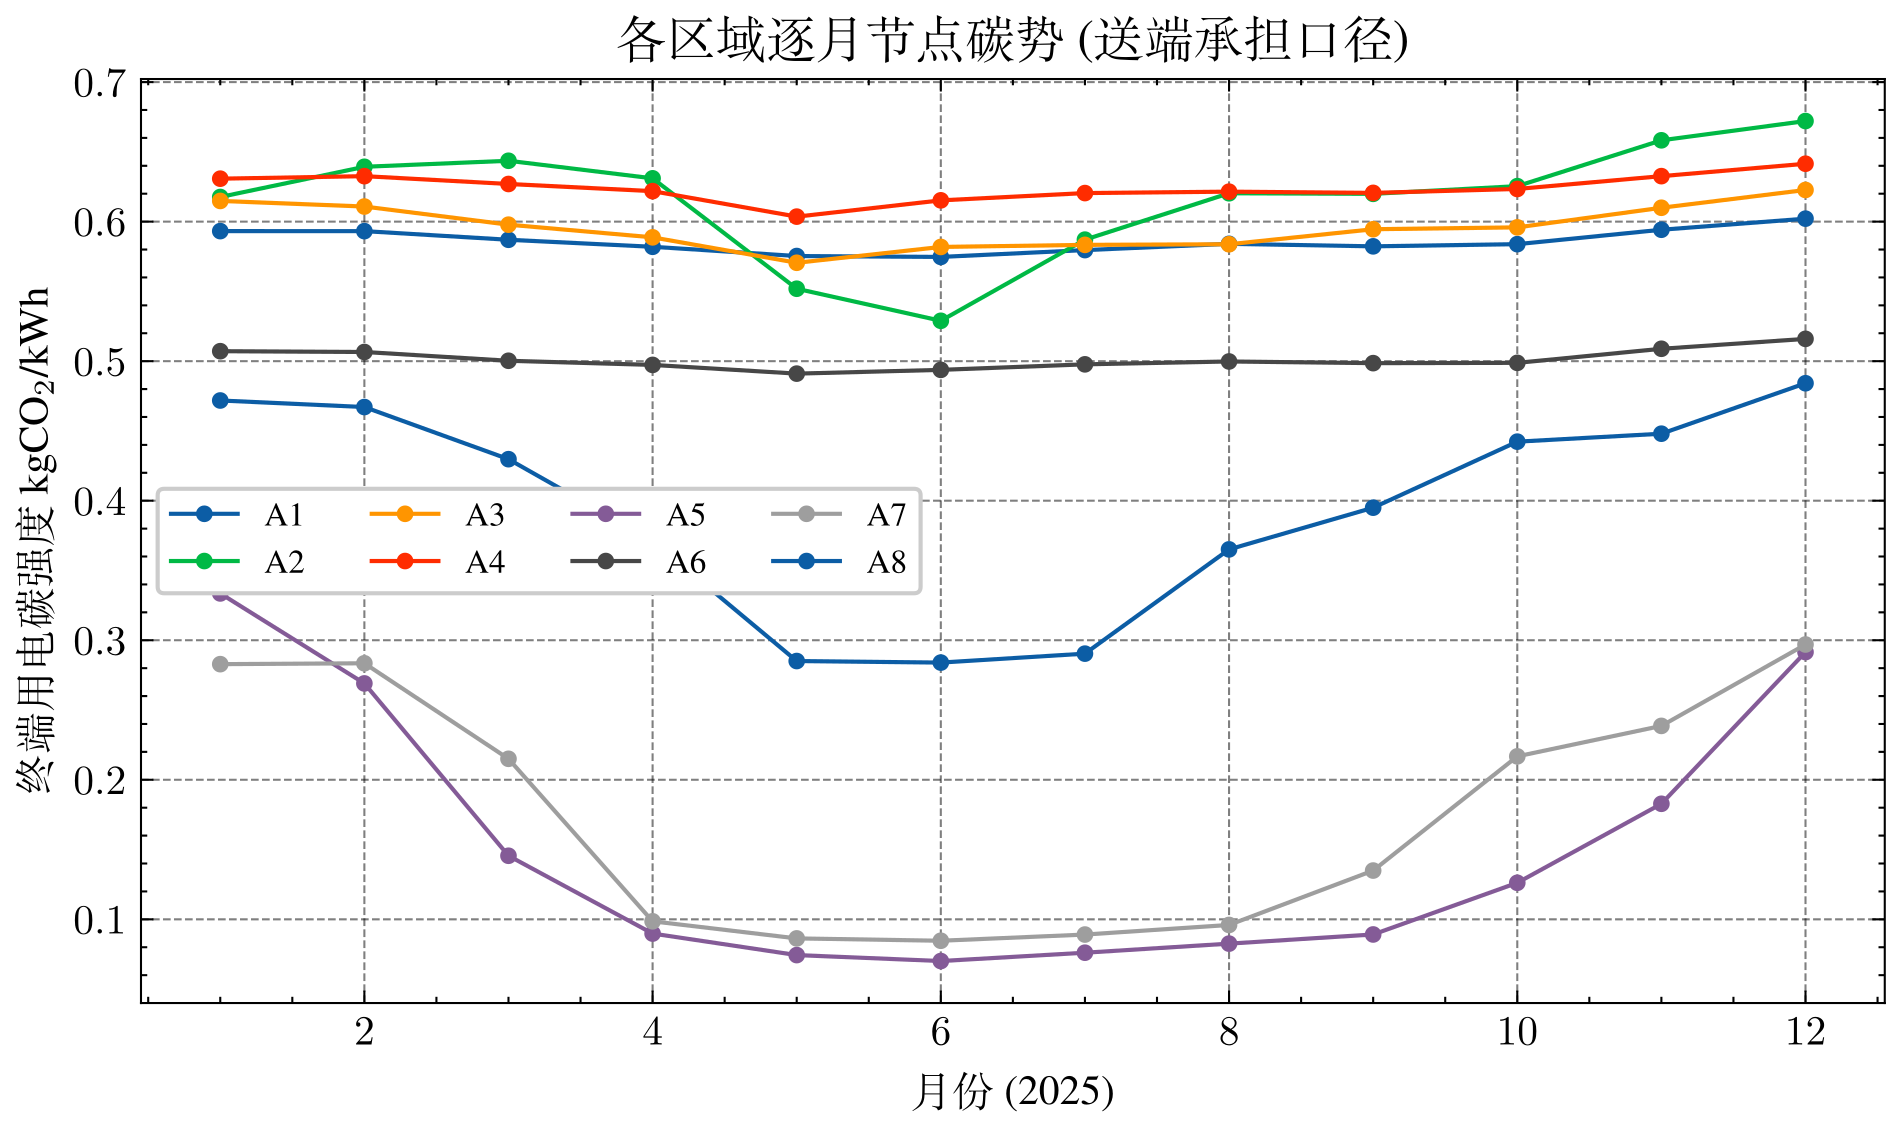
\includegraphics[width=0.92\textwidth]{fig_q2_rho_monthly.png}
\caption{各区域 2025 年逐月节点碳势（送端承担口径）。A4、A2 全年偏高，A5、A7 因水电占比高而显著偏低。}
\label{fig:rho}
\end{figure}

\begin{figure}[htbp]
\centering
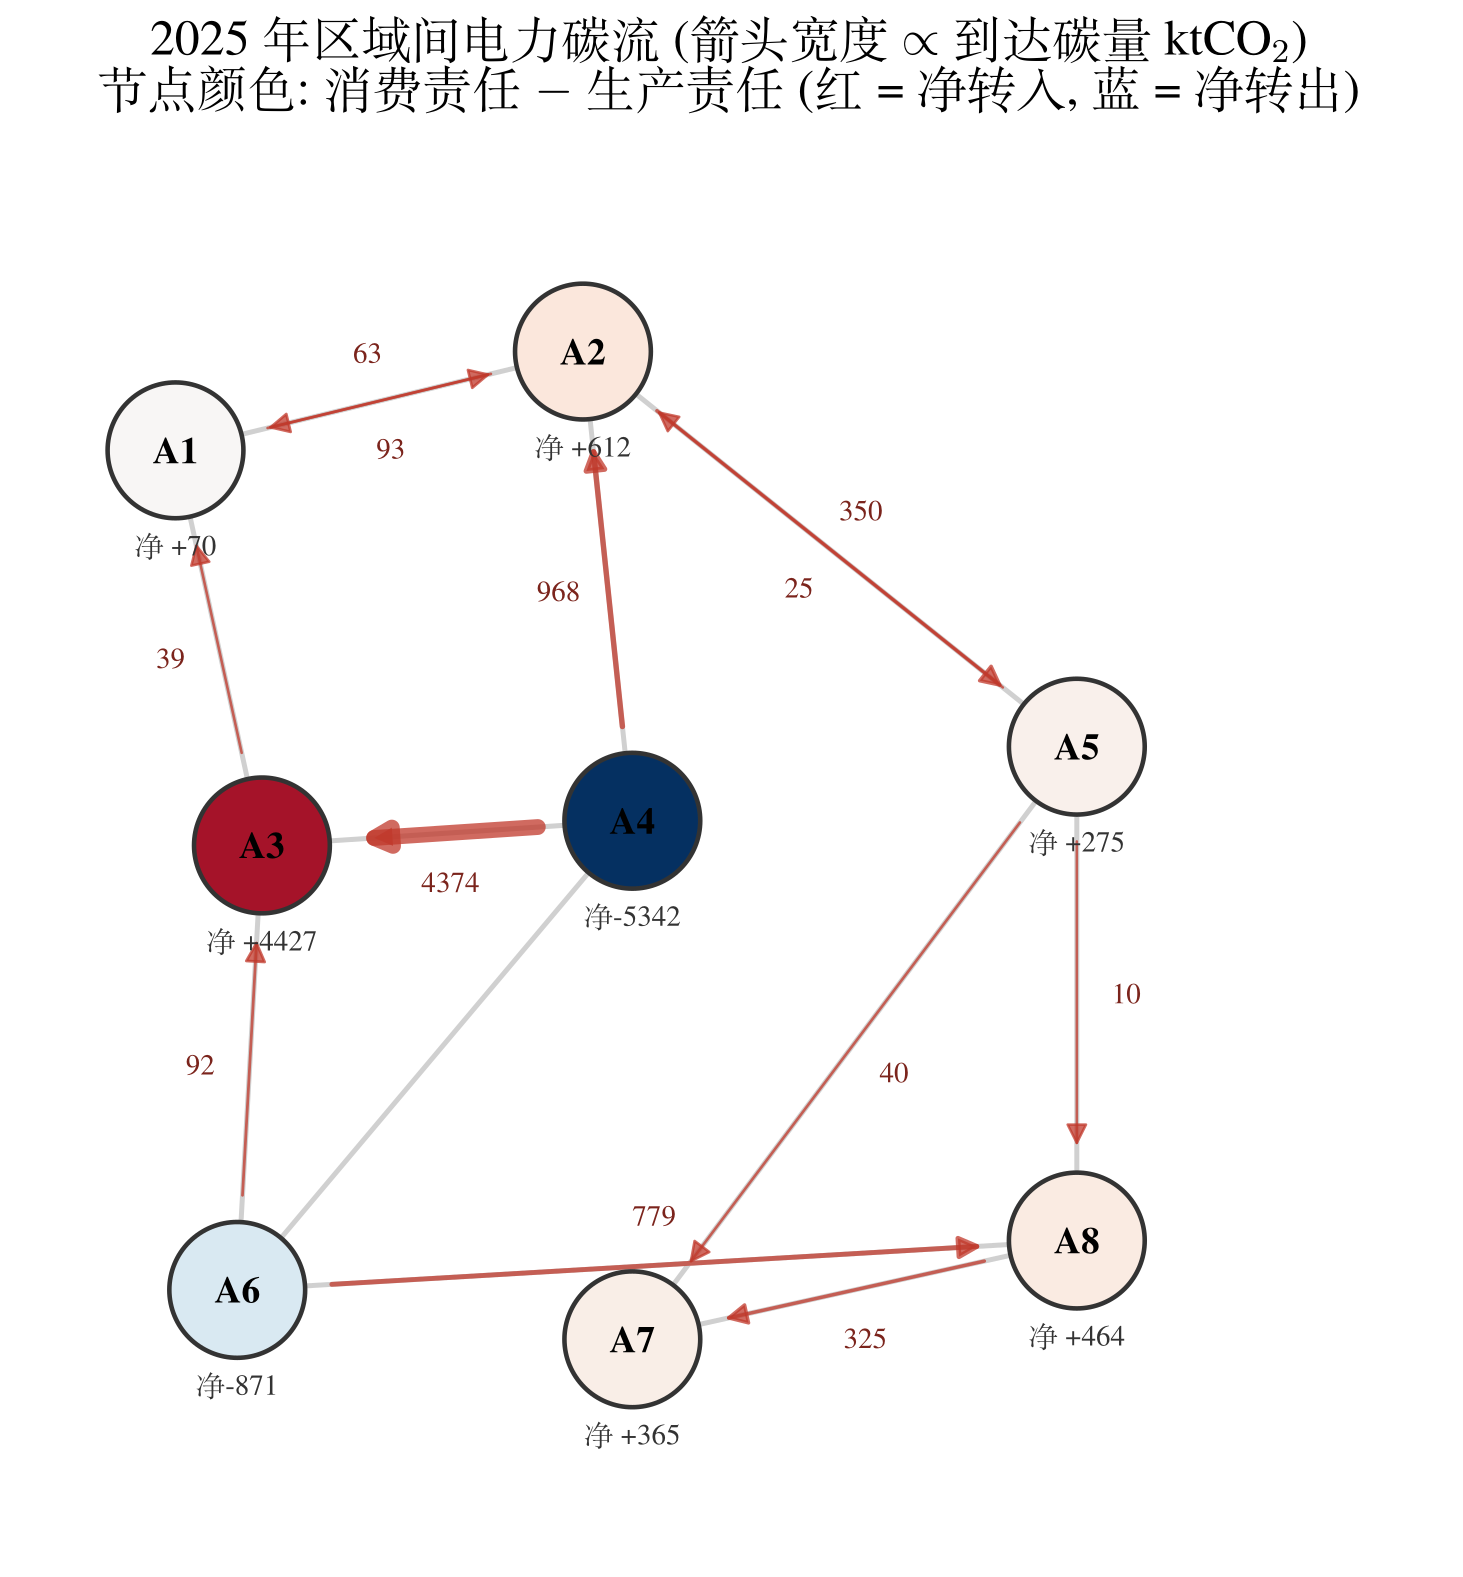
\includegraphics[width=0.88\textwidth]{fig_q2_carbon_flow_network.png}
\caption{2025 年区域间电力碳流与净责任格局。箭头宽度正比于到达碳量 $F_{j\to i}$（ktCO$_2$）；节点颜色为 $C^+_i-P^+_i$（红=净转入）。主路径为 A4$\to$A3（4374\,kt）。}
\label{fig:cfnet}
\end{figure}

\begin{figure}[htbp]
\centering
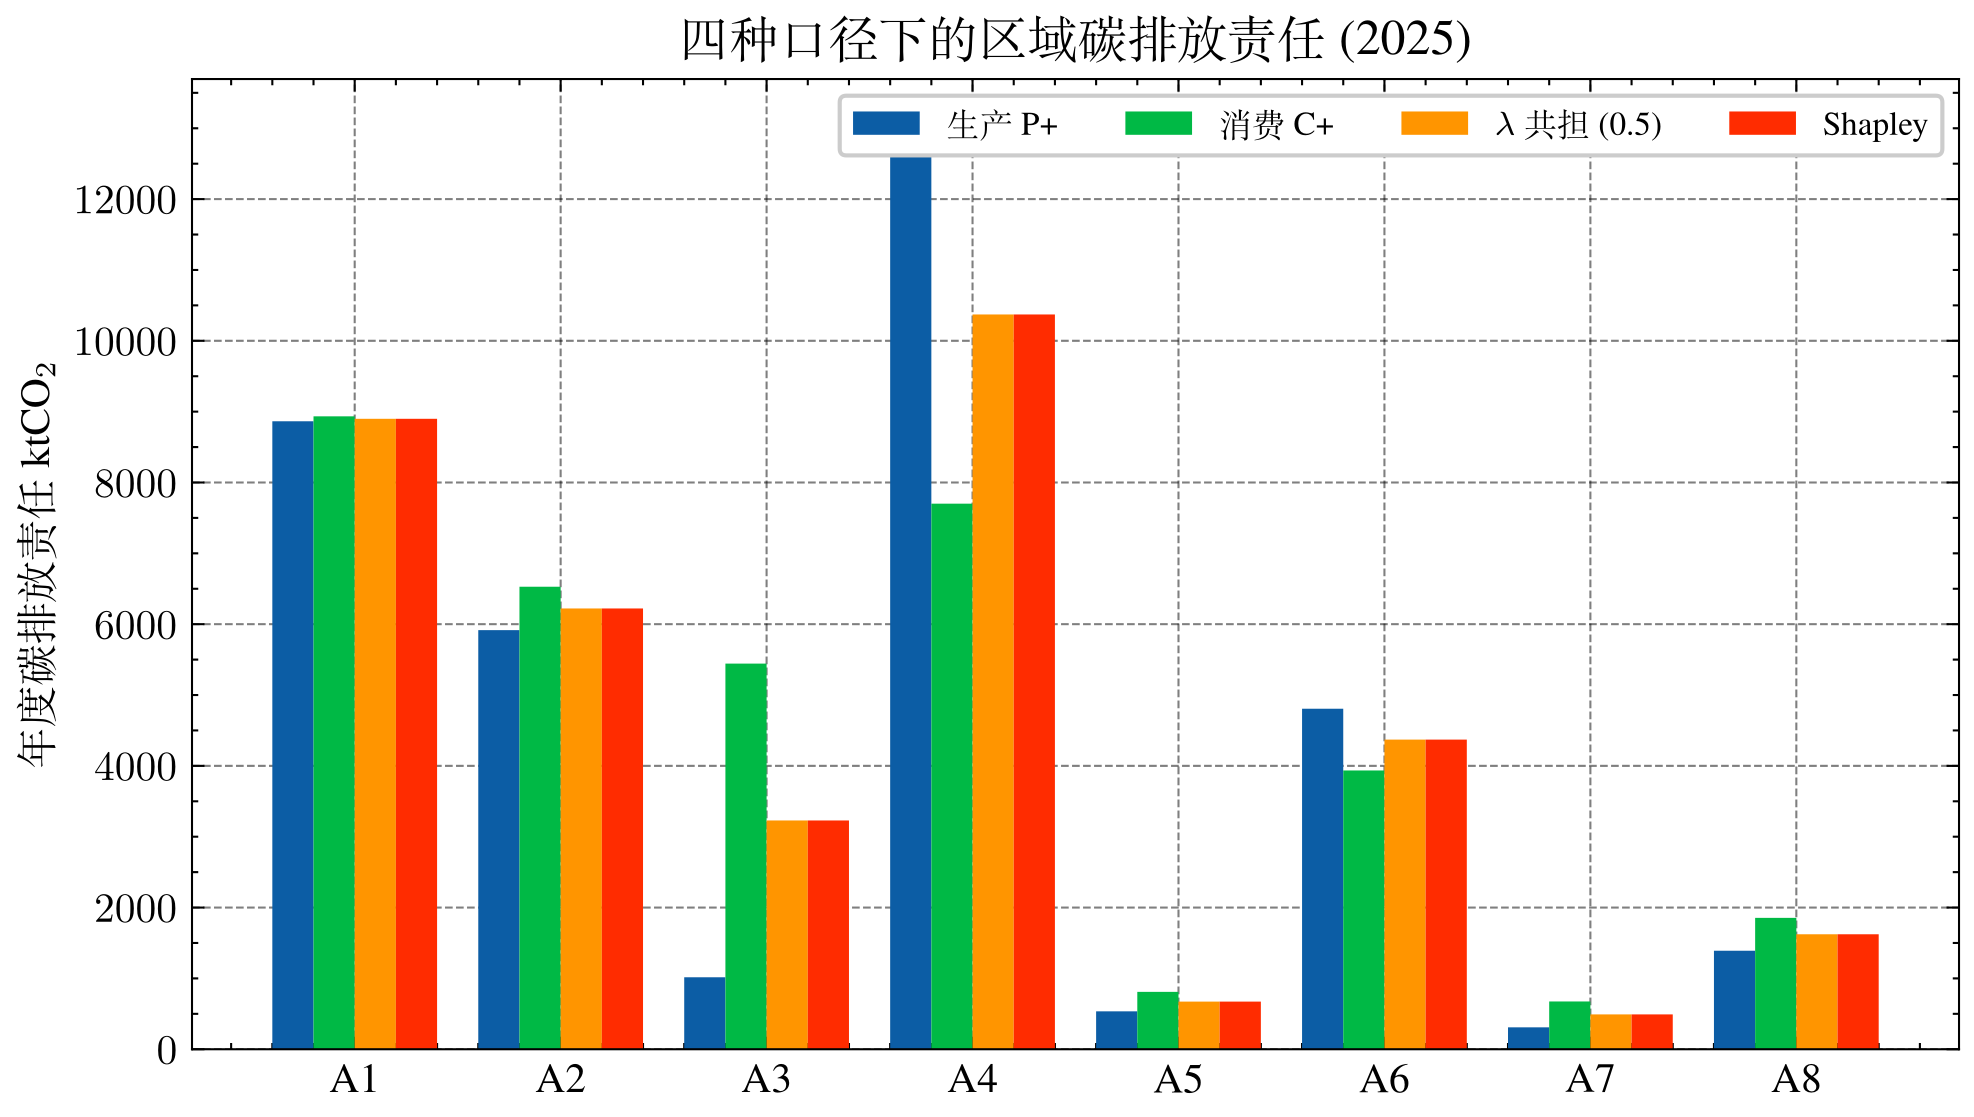
\includegraphics[width=0.92\textwidth]{fig_q2_responsibility_shapley.png}
\caption{四种口径下的区域碳排放责任（2025）。$\lambda=0.5$ 与 Shapley 柱高重合，验证五五分成的博弈含义。}
\label{fig:resp}
\end{figure}

\begin{table}[htbp]
\centering
\caption{2025 年区域碳排放责任与 Shapley 共担（ktCO$_2$）}
\label{tab:resp}
\resizebox{\textwidth}{!}{
\begin{tabular}{lrrrrr}
\toprule
区域 & $P^+$ & $C^+$ & $\lambda=0.3$ & $\lambda=0.5$ & Shapley \\
\midrule
A1 & 8864.13 & 8933.65 & 8912.79 & 8898.89 & 8898.89 \\
A2 & 5916.00 & 6528.19 & 6344.53 & 6222.09 & 6222.09 \\
A3 & 1015.92 & 5443.21 & 4115.02 & 3229.56 & 3229.56 \\
A4 & 13042.69 & 7700.88 & 9303.42 & 10371.78 & 10371.78 \\
A5 & 535.57 & 810.34 & 727.91 & 672.96 & 672.95 \\
A6 & 4806.71 & 3935.37 & 4196.77 & 4371.04 & 4371.04 \\
A7 & 309.29 & 674.40 & 564.87 & 491.84 & 491.85 \\
A8 & 1390.50 & 1854.76 & 1715.48 & 1622.63 & 1622.63 \\
合计 & 35880.81 & 35880.80 & --- & --- & 35880.80 \\
\bottomrule
\end{tabular}}
\end{table}

\section{问题三：区域碳预算与五年项目组合}

\subsection{预算分解}

全省消费侧年度上限 $\overline E_y$ 为硬约束。区域软预算采用惯性份额与公平份额的凸组合\cite{Raupach2014sharing,Zhou2016carbon,Wang2013regional}
\begin{equation}
B_{i,y}=\bigl[w_y\pi_i+(1-w_y)d_{i,y}\bigr]\overline E_y,
\label{eq:budget}
\end{equation}
其中 $\pi_i$ 为 2025 年 $C^+$ 份额，$d_{i,y}$ 为当年需求份额，$w_y$ 由 2026 年的 0.85 线性降到 2030 年的 0.65。超额 $b_{i,y}=\max(0,E_{i,y}-B_{i,y})$ 按 0.2 百万元/kt（约 200 元/tCO$_2$）计罚。

\subsection{投资—运行耦合 MILP}

决策变量为项目 $p$ 在年份 $t$ 的开工规模 $x_{p,t}$（通道升级为 0-1）。运行层包含本地电源上限、省外输入年容量、通道容量与问题一校正后的 $\eta_e$，以及最低供能率。碳核算按附件 4B 的官方简化式
\begin{equation}
E_{i,y}=\rho_i\kappa_y(D_{i,y}-G^{\mathrm{PV}}_{i,y})+0.045\,G^{\mathrm{PV}}_{i,y}-A_{i,y},
\label{eq:E}
\end{equation}
交通电气化新增用电计入 $D$，燃油替代计入直接减排 $A$，不重复计算。$\rho_i$ 取问题二 2025 年终端碳强度。目标为
\begin{equation}
\min\sum_{p,t}\frac{c_p x_{p,t}}{(1+r)^{t-2026}}
+0.2\sum_{i,y}b_{i,y}
+10\sum_{i,y}(D_{i,y}-s_{i,y}),
\label{eq:obj}
\end{equation}
主方案折现率 $r=0$。约束包括总规模与年开工上限、五类施工资源、年度投资上限、互斥、协同触发的 McCormick 线性化。该结构属于多年期投资—运行耦合的发电扩张规划范式\cite{Koltsaklis2018generation}。

为避免把 MILP 写成“黑箱出一个数”，同时报告两个可手算理解的对照：无项目（$x=0$）以及按 2030 年单位减排成本升序、逐年补到刚好满足省级上限的贪心可行解。

\subsection{主方案、贪心与无项目}

无项目在 2026 年碳量为 34874.6\,kt，仍低于上限 35200；自 2027 年起越限，五年累计 \textbf{567\,kt}。贪心投资 976.2 百万元即可全年不越限，入选 6 个项目，与 MILP 的项目—年 Jaccard 为 0.625。MILP 主方案总投资 \textbf{985.5} 百万元，目标值 1923.0（其中区域预算罚 913.7），入选 7 个项目：交通电气化 P07/P15/P23/P31 与分布式光伏 P08/P12/P16。通道升级 P33—P35 未入选——因为\eqref{eq:E}不含潮流，通道不直接减排，而主方案缺供为 0，升级没有供能方面的必要。碳裕度 2026—2030 年为 325.4、56.0、3.1、0、0\,kt，后期上限是绑定约束。影子价格 2029 年为 0.60、2030 年为 3.162 百万元/kt。投资上限在 0.8—1.2 倍时 Jaccard 恒为 1；碳上限再收紧 3\% 则不可行，放宽 3\% 则方案重构（Jaccard 0）。优先序与单位减排成本表一致：交通电气化先于光伏，光伏先于工业节能。

\begin{figure}[htbp]
\centering
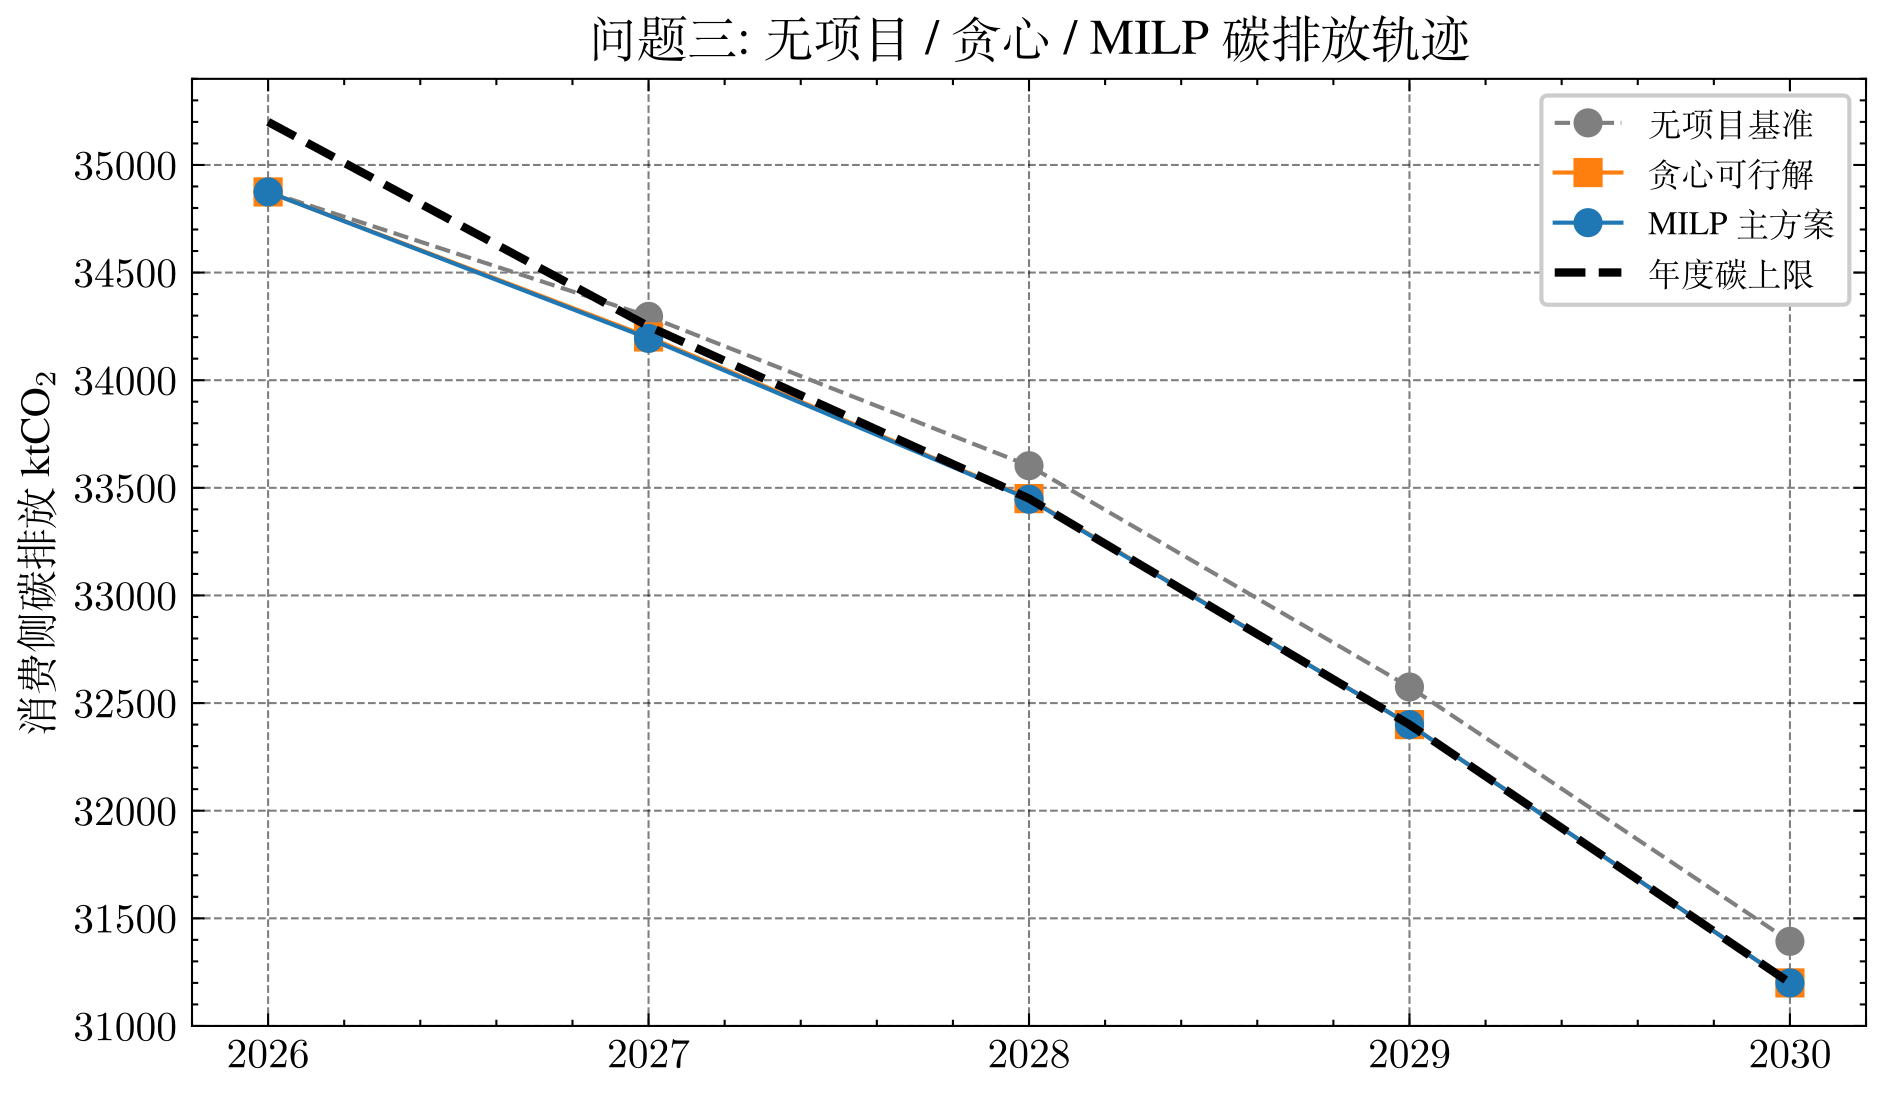
\includegraphics[width=0.92\textwidth]{fig_q3_no_project.png}
\caption{问题三：无项目、贪心与 MILP 的消费侧碳轨迹。2026 年三类重合（项目尚未投运）；无项目自 2027 年起越限；贪心与 MILP 在 2028—2030 年贴上限运行。}
\label{fig:noproj}
\end{figure}

\begin{figure}[htbp]
\centering
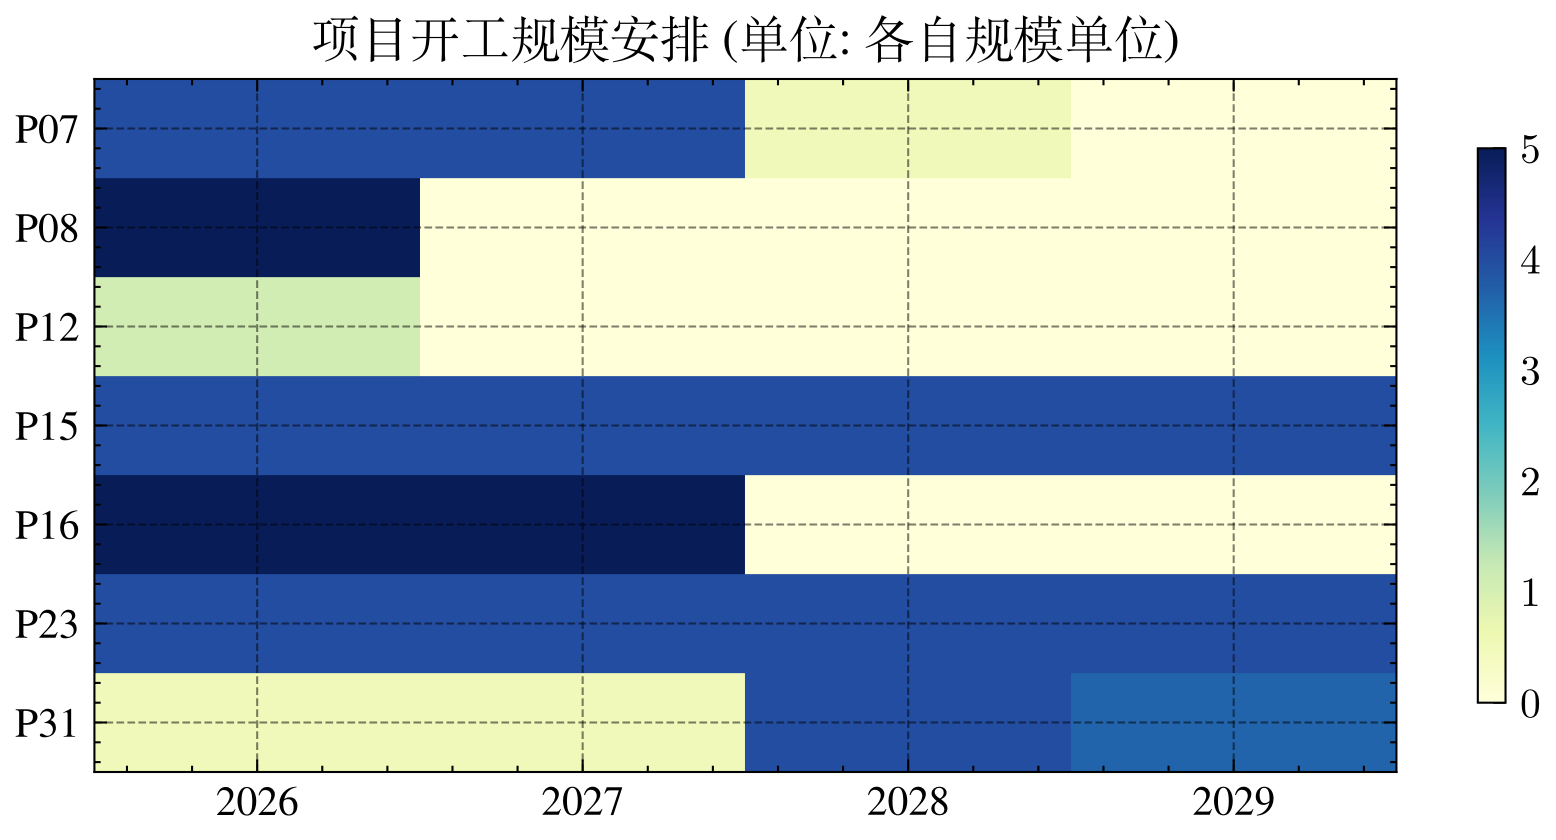
\includegraphics[width=0.92\textwidth]{fig_q3_schedule.png}
\caption{五年项目开工规模安排（主方案）。投资集中于 2026—2028 年；通道升级未入选。}
\label{fig:sched}
\end{figure}

\begin{table}[htbp]
\centering
\caption{无项目、贪心可行解与 MILP 主方案比较}
\label{tab:base}
\begin{tabular}{lccccc}
\toprule
方案 & 投资 & 五年总越限 & 区域超额合计 & Jaccard & 项目数 \\
\midrule
无项目 & 0 & 567.0 & 5078.2 & 0 & 0 \\
贪心（补到上限） & 976.2 & 0 & 4637.0 & 0.625 & 6 \\
MILP 主方案 & 985.5 & 0 & 4568.4 & 1 & 7 \\
\bottomrule
\end{tabular}
\end{table}

\begin{table}[htbp]
\centering
\caption{折现率、区域预算罚、缺供罚与惯性权重的敏感性}
\label{tab:q3sens}
\begin{tabular}{lcccc}
\toprule
设定 & 目标 & 投资 & Jaccard & 区域超额 \\
\midrule
折现率 0（主方案） & 1923.0 & 985.5 & 1.000 & 4568.4 \\
折现率 8\% & 1862.2 & 986.3 & 0.696 & 4606.7 \\
区域预算罚 0.1 & 1463.0 & 976.7 & 0.900 & 4625.2 \\
区域预算罚 0.4 & 2826.2 & 1013.4 & 0.652 & 4472.5 \\
VOLL $=5,10,20$ & 1923.0 & 985.5 & 1.000 & 4568.4 \\
惯性权重全期 0.50 & 2824.3 & 985.5 & 1.000 & 9075.2 \\
惯性权重全期 0.85 & 1678.5 & 998.7 & 0.810 & 3280.3 \\
\bottomrule
\end{tabular}
\end{table}

表\ref{tab:q3sens}可直接回答“这些数是不是拍的”。缺供罚在 5—20 范围内方案不变，因为最低供能率已是硬约束、缺供为 0。区域预算罚只在 977—1013 百万元之间微调投资。更公平的惯性权重几乎只增加罚项、不改实物方案——绑定约束是省级上限而不是区域预算。8\% 折现几乎不改变五年投资总额，但开工年 Jaccard 降至 0.696，说明折现改变的是“哪一年花钱”，不是“买哪类项目”。主方案取 $r=0$，与附件投资上限同口径。

\section{问题四：送端碳不确定与鲁棒滚动}

\subsection{冲击如何传到消费侧}

问题三方案在基准因子路径上贴着 2028—2030 年上限运行，对送端变“脏”没有余量。记 $\xi_{j,y}$ 为接入区 $j$ 的因子乘数。若把进口偏差直接加到接入区碳账，会与 $\rho\cdot\kappa$ 基线双计。与问题二一致的传导是：先用 2025 年份额得到“源自 $j$ 的消费电量” $W_{j,y}=\sum_i(D_{i,y}-G^{\mathrm{PV}}_{i,y})S_{ij}$，再
\begin{equation}
\Delta E_y=\kappa_y\sum_j \bar e_j(\xi_{j,y}-1)W_{j,y}.
\label{eq:dE}
\end{equation}
$S_{ij}$ 冻在 2025 年是强假设。将传导改为“只计接入区进口电量、忽略转供”时，S3 情景 2030 年增量由 454.5\,kt 变为 437.8\,kt（相对偏差 $-3.7\%$）；若把 $S$ 再向 A4 集中 20\%，则升至 495.7\,kt。主方案对是否追踪转供不敏感，对枢纽进一步集中更敏感。后续应在规划潮流上重解碳流；在未更新前，鲁棒方案覆盖的是因子冲击而不是 $S$ 的漂移。

\subsection{\texorpdfstring{压力测试、$\Gamma$-鲁棒与滚动}{压力测试、鲁棒与滚动}}

在固定问题三方案下，S3 情景 2028/2029/2030 年越限 195.4、338.5、454.5\,kt，预算集最坏合计 1125.46\,kt。对 $\xi$ 采用预算不确定集\cite{Bertsimas2004price}
\begin{equation}
\bigl\{\boldsymbol z:\ 0\le z_j\le 1,\ \textstyle\sum_j z_j\le \Gamma_y\bigr\},
\label{eq:budgetset}
\end{equation}
内层最大增量对偶化为 $\Gamma_y\pi_y+\sum_j\mu_{j,y}$，嵌回 MILP 即静态鲁棒。扫描 $\tau$（$\Gamma_y$ 乘子）得到 price-of-robustness（表\ref{tab:gamma}）：$\tau=0$ 投资 985.5、最坏越限 1125.46；$\tau=1$ 投资 4848.8、残余 18.17；$\tau\ge 1.5$ 投资饱和在 5160.4。

\begin{table}[htbp]
\centering
\caption{$\Gamma$ 缩放下的投资与最坏越限（price of robustness）}
\label{tab:gamma}
\begin{tabular}{ccc}
\toprule
$\tau$ & 投资（百万元） & 最坏情景总越限（kt） \\
\midrule
0.0 & 985.5 & 1125.46 \\
0.5 & 3387.4 & 341.07 \\
1.0 & 4848.8 & 18.17 \\
1.5 & 5160.4 & 18.21 \\
2.0 & 5160.4 & 18.21 \\
\bottomrule
\end{tabular}
\end{table}

两阶段可调鲁棒把 2026—2027 开工作为此地决策、后期作为观望决策\cite{BenTal2004adjustable}，用顶点加列求解\cite{Zeng2013solving}，两轮目标 5251.5$\to$6522.4。滚动则在 S3 路径上逐年用已观测 $\xi$，对未观测年保留 $\Gamma$-鲁棒\cite{Silvente2015rolling}。

\begin{figure}[htbp]
\centering
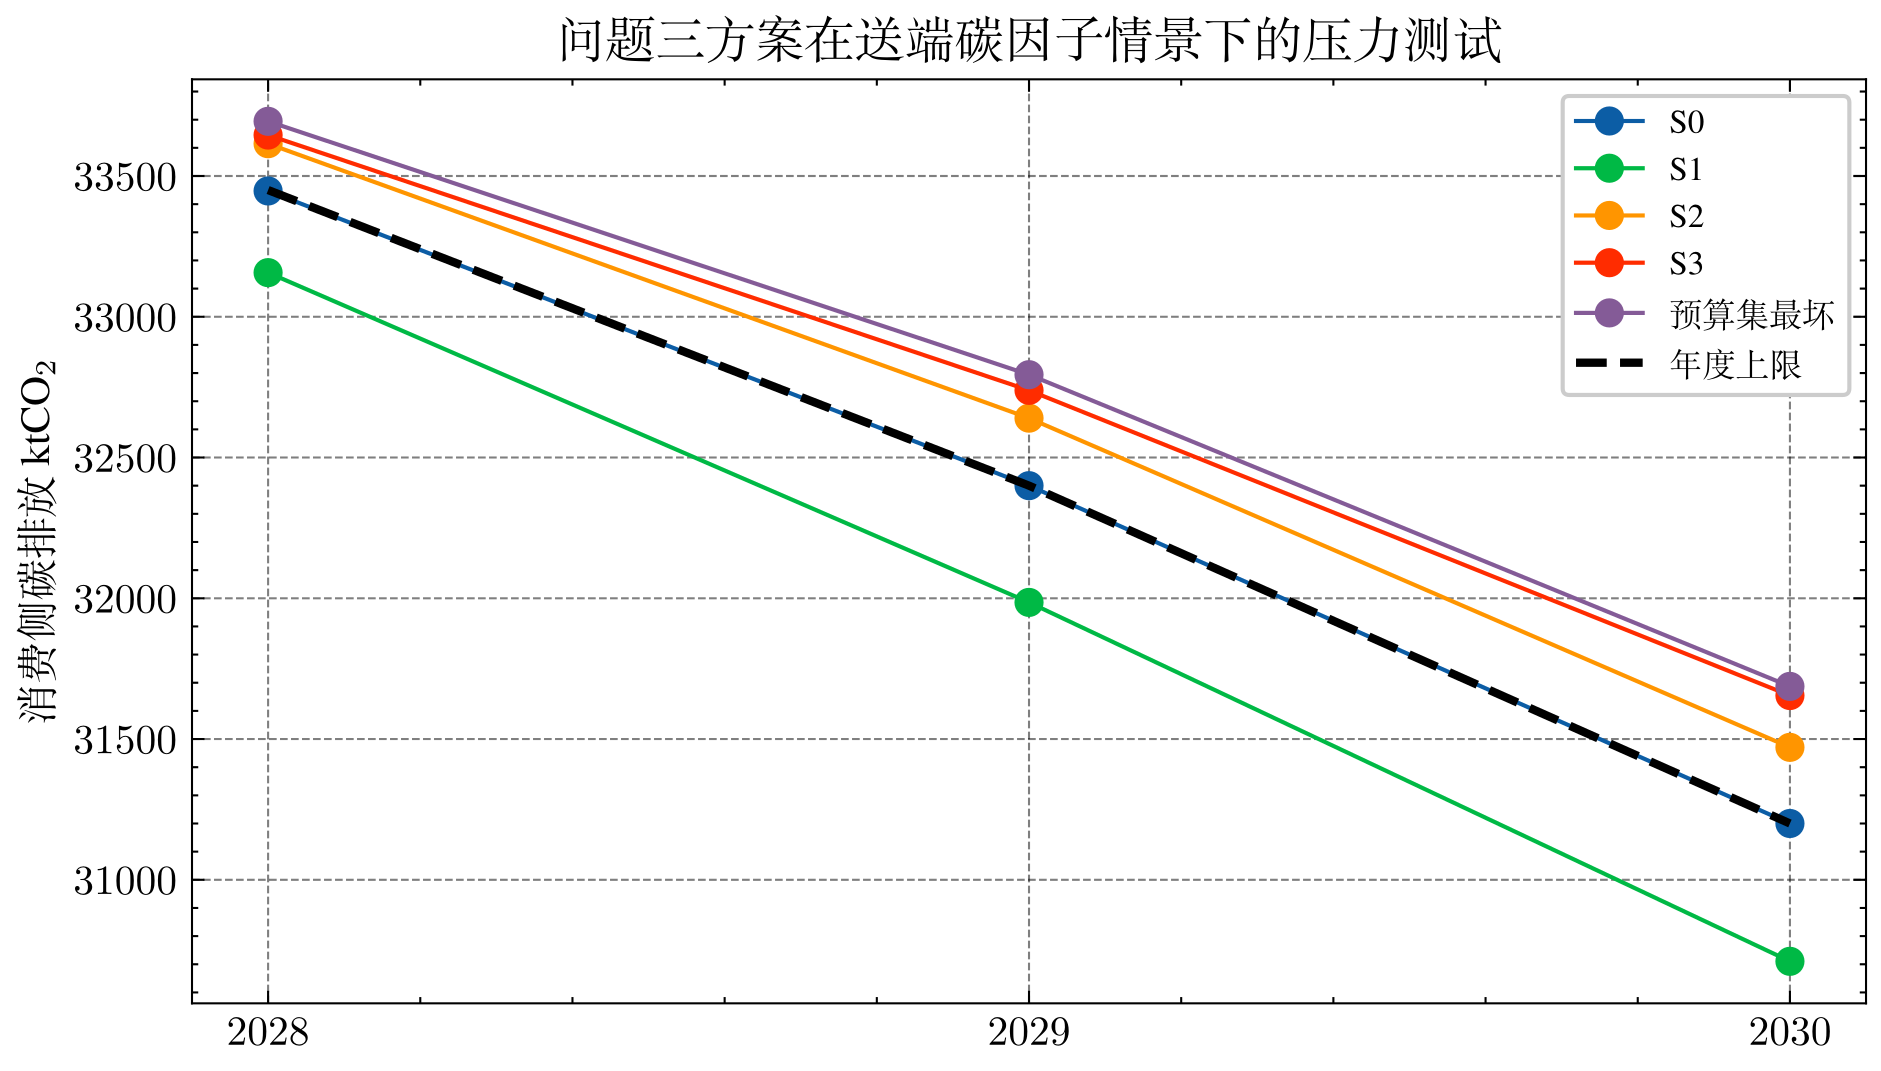
\includegraphics[width=0.92\textwidth]{fig_q4_stress.png}
\caption{问题三方案在送端碳因子情景下的压力测试。S3 情景 2030 年越限 454.5\,kt。}
\label{fig:stress}
\end{figure}

\begin{figure}[htbp]
\centering
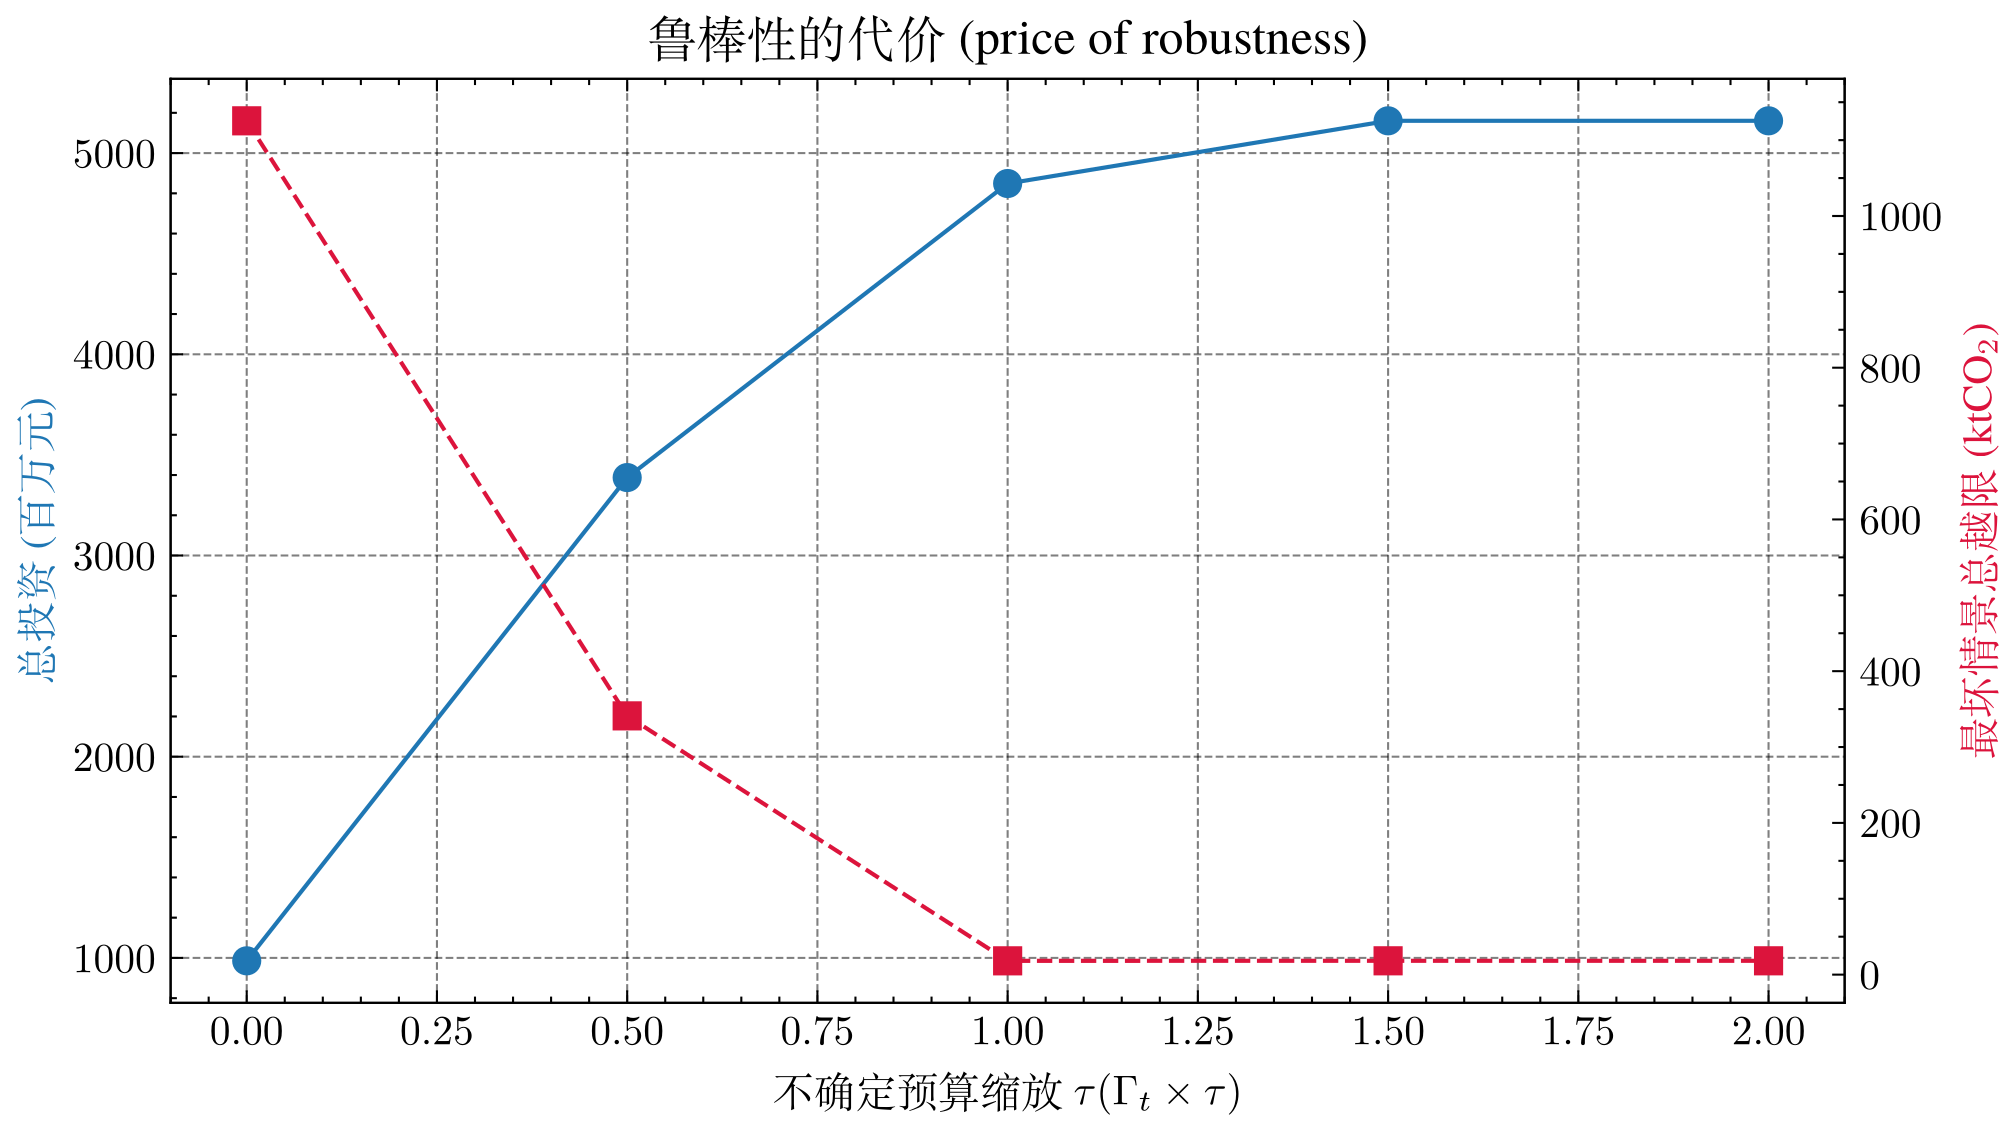
\includegraphics[width=0.92\textwidth]{fig_q4_por.png}
\caption{鲁棒性的代价：不确定预算缩放 $\tau$ 与投资、最坏越限。$\tau=1$ 时溢价 3863.3 百万元，残余越限 18.17\,kt。}
\label{fig:por}
\end{figure}

\begin{table}[htbp]
\centering
\caption{确定性、静态鲁棒与稳健滚动对照}
\label{tab:three}
\begin{tabular}{lcccc}
\toprule
方案 & 投资 & S3-2028 & S3-2029 & S3-2030 \\
\midrule
确定性（问题三） & 985.5 & 195.4 & 338.5 & 454.5 \\
静态鲁棒（$\tau=1$） & 4848.8 & 0 & 0 & 0 \\
稳健滚动（S3 路径） & 4848.8 & 0 & 0 & 0 \\
\bottomrule
\end{tabular}
\end{table}

\begin{figure}[htbp]
\centering
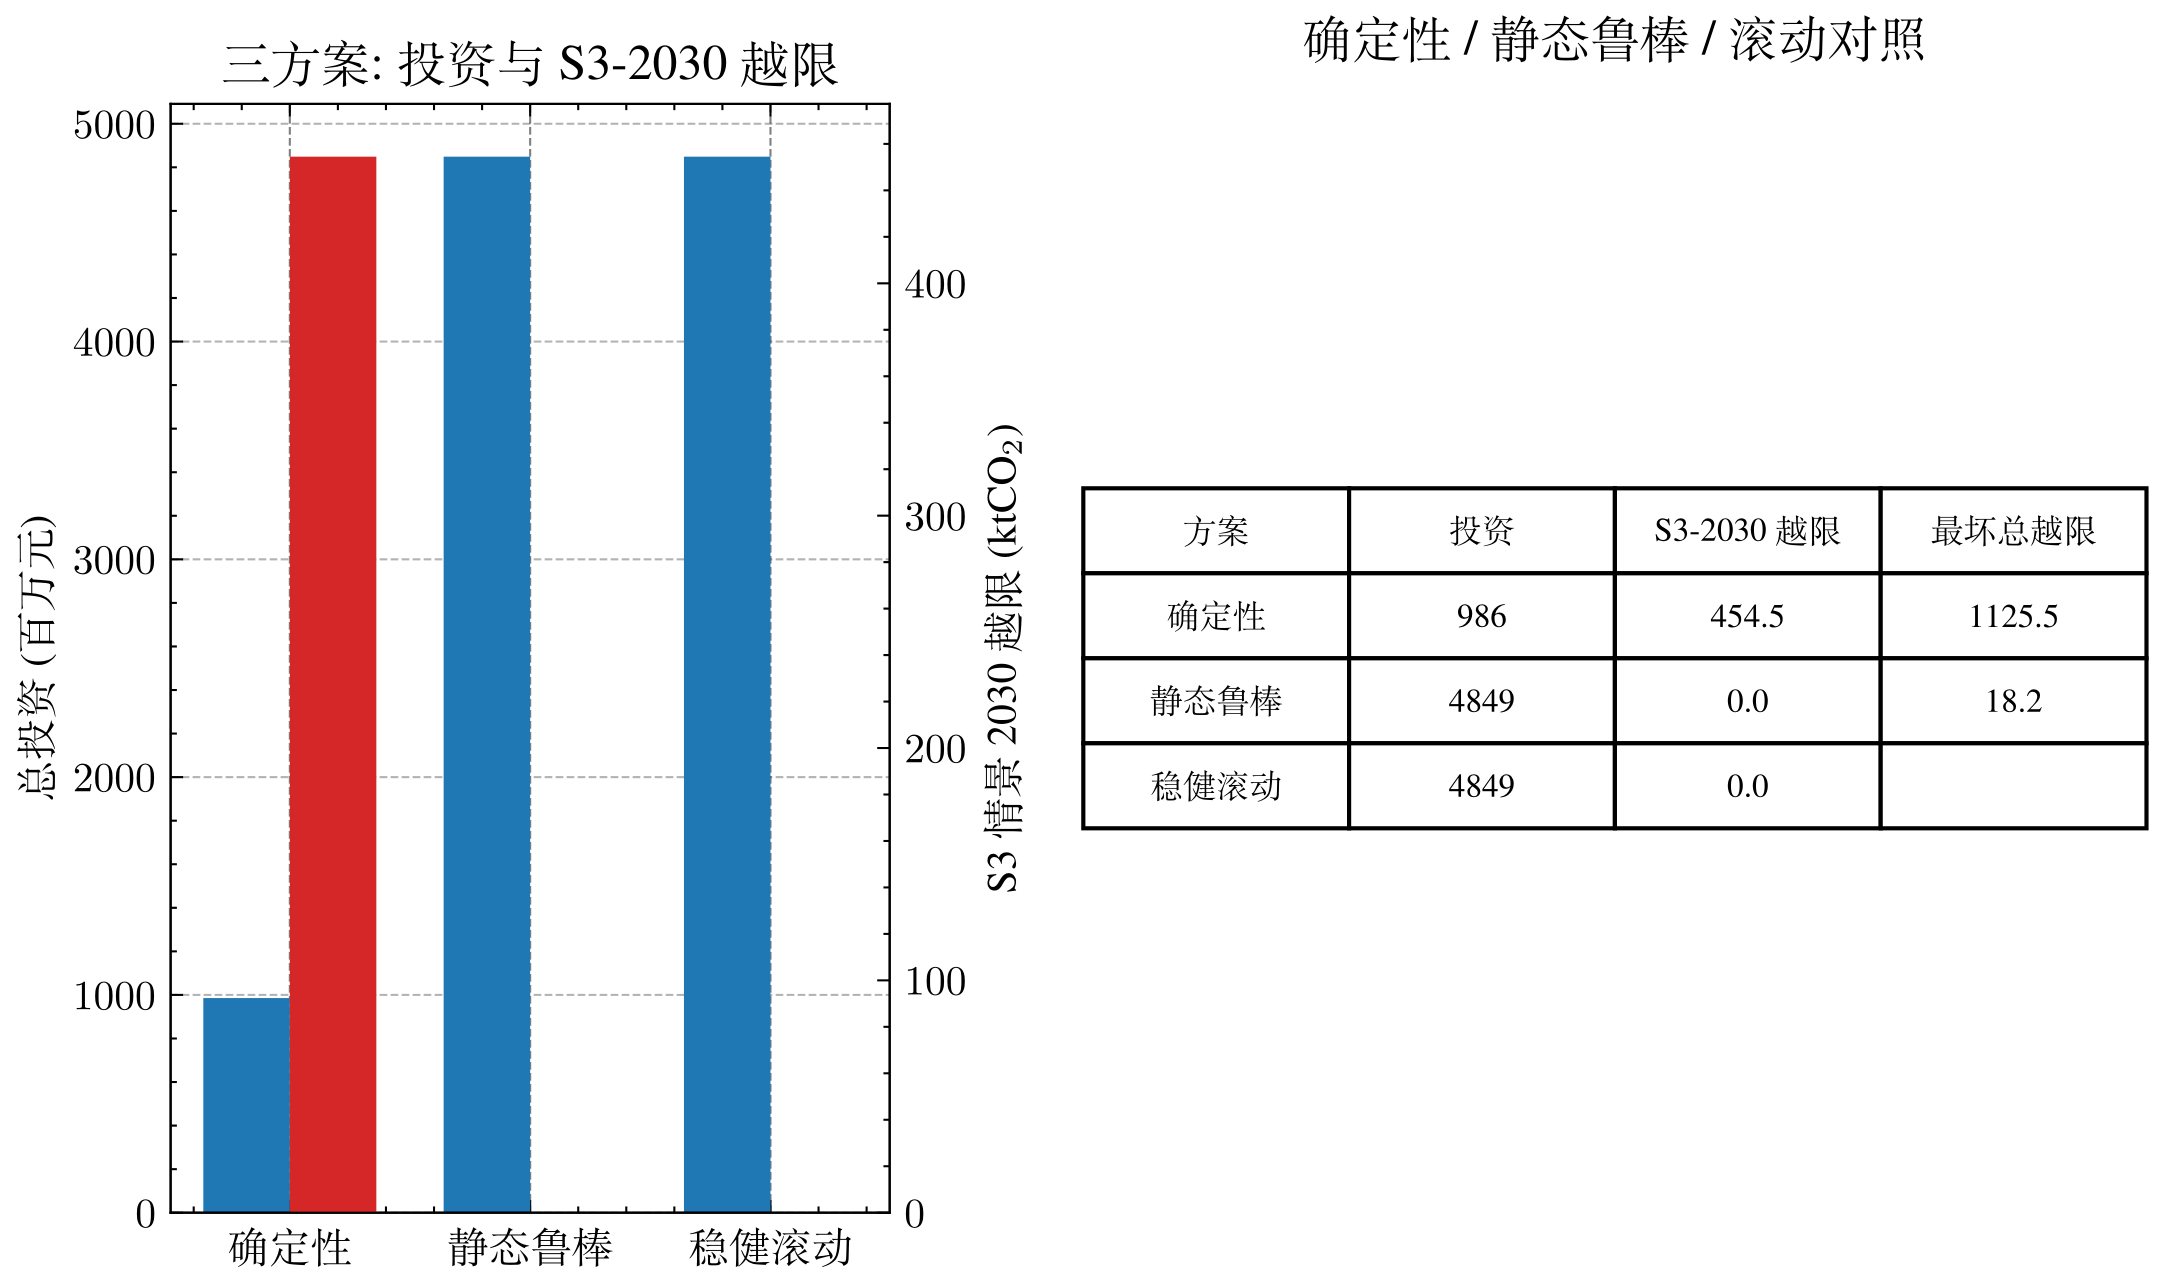
\includegraphics[width=0.92\textwidth]{fig_q4_three_schemes.png}
\caption{确定性、静态鲁棒与稳健滚动：投资与 S3-2030 越限。静态鲁棒最坏总越限仍余 18.17\,kt；滚动在本规则下实物投资与静态鲁棒相同。}
\label{fig:three}
\end{figure}

表\ref{tab:three}必须读完整：静态鲁棒在 S3 下已经零越限，最坏情景仍余 18.17\,kt。稳健滚动在 S3 下同样零越限，\textbf{实物总投资同为 4848.8}——因为第一阶段已按两阶段鲁棒锁定，且未观测年始终按 $\Gamma=1$ 设防；S0/S1/S3 三条观测路径下总投资相同。滚动的可测量价值是剩余期目标 6130.6$\to$5614.0 百万元，以及 2028 年决策时累计投资仅为 3760.4、尚未锁死全部五年。不能把本次数值实验写成“观测到温和路径就少花了钱”。若主管部门在观测后下调 $\tau$，滚动框架允许少开工，那是政策选择，不是本文已经实现的投资节约。日常执行因此推荐滚动机制，压力底线用静态鲁棒，确定性方案不能直接下达。

\section{问题五：决策咨询报告}

{\heiti 关于“十五五”电力低碳转型的决策建议}

{\kaishu （呈省级能源主管部门）}

\vspace{0.3em}
对 2025 年多源监测数据的守恒校验共识别异常与口径不一致 23 处，包括月度与年度两套系统最大 8.7\% 的口径差、通道 E10“受端大于送端”、E03 单月隐含线损 17.5\%，以及 4 处缺失。加权最小二乘调和后，通道损耗总体与工程记录相符，但 E05 实际约 0.0135（工程值 0.020）。E10 年度送端、A5 终端用电、A4 省外输入对全网校正影响最大，建议优先做关口与年度汇总的口径对齐。

碳随电走。A4 终端碳强度 0.62\,kgCO$_2$/kWh，A5 仅 0.15。纯受电区 A3 的消费责任是生产责任的 5.36 倍，主碳流 A4$\to$A3 达 4374\,kt。单一口径考核必然失真。建议以生产—消费五五共担作为区域双控基准（该口径与通道碳转移博弈的 Shapley 值一致，全省总量守恒），区域预算按“现状份额走向公平份额”五年过渡。

五年碳上限可在总投资 985.5 百万元内全部达标，优先序为交通电气化、分布式光伏、工业节能。2030 年碳约束影子价格约 3.16 百万元/kt，可作为补贴与区域预算交易的定价锚。若碳上限再收紧 3\%，现有项目库无解，减排潜力已到天花板，需要提前储备第二批项目。通道升级在现行碳口径下不减排，主方案未安排，避免把投资误投到“看起来像电网、算碳时却不算数”的工程。

省外来电若走高碳路径（S3），2030 年将超上限 454.5\,kt。要把五年方案一次性做成对预算集免疫，投资需升至 4848.8 百万元，仍可能余 18\,kt 缺口。滚动调控——每年根据已观测的送端结构重解剩余期、对未观测年保留鲁棒——在 S3 下可零越限，剩余期成本随信息到达由 6130.6 降至 5614.0 百万元。需要讲清楚：滚动并不自动比静态鲁棒少花钱；它的意义是不把五年开工一次性锁死，并保留观测后下调设防强度的接口。建议以滚动为工作机制，以静态鲁棒为压力底线预案，每年三季度更新碳因子区间并调整次年开工。

\section{模型评价、局限性与结论}

本文把赛题拆成有文献出处的四段标准问题：数据调和、碳排放流、投资—运行 MILP、预算鲁棒与滚动，并补了无项目/贪心、Shapley 枚举和参数敏感性，避免“求解器给出一个孤立最优”。主要局限如下。第一，$S_{ij}$ 冻到 2030 年，S3-2030 增量对忽略转供偏差约 4\%，对枢纽再集中更敏感。第二，官方碳公式不含潮流，通道升级的规划价值被系统性低估。第三，VOLL、5\% 损耗先验、0.2 的区域罚都是建模选择，已各做两组敏感性，结论方向稳定但绝对值会动。第四，稳健滚动在“未来年始终 $\Gamma=1$”下与静态鲁棒投资重合，不可夸大信息价值。第五，责任共担没有唯一“正确”的 $\lambda$，0.5 的特殊地位来自 Shapley 恒等式，政策上仍可在 0.3—0.7 之间讨论。

结论可以收成四句话。先校准 2025 年电量，再谈碳账。考核用五五共担，承认 A4$\to$A3 的碳转出。基准路径 985.5 百万元可以守住五年上限，优先交通电气化与光伏。送端冲击用滚动机制应对，用静态鲁棒做底线，不要把确定性方案直接变成年度计划。

\begin{thebibliography}{21}
\bibitem{Crowe1996data} Crowe C M. Data reconciliation — Progress and challenges[J]. Journal of Process Control, 1996, 6(2-3): 89-98.
\bibitem{Narasimhan1999data} Narasimhan S, Jordache C. The Importance of Data Reconciliation and Gross Error Detection[M]//Data Reconciliation and Gross Error Detection. Elsevier, 1999: 1-31.
\bibitem{Schweppe1970power} Schweppe F C, Wildes J. Power System Static-State Estimation, Part I: Exact Model[J]. IEEE Transactions on Power Apparatus and Systems, 1970, PAS-89(1): 120-125.
\bibitem{Abur2004power} Abur A, Expósito A G. Power System State Estimation: Theory and Implementation[M]. CRC Press, 2004.
\bibitem{deChalendar2021physics} de Chalendar J A, Benson S M. A physics-informed data reconciliation framework for real-time electricity and emissions tracking[J]. Applied Energy, 2021, 304: 117761.
\bibitem{Bialek1996tracing} Bialek J. Tracing the flow of electricity[J]. IEE Proceedings - Generation, Transmission and Distribution, 1996, 143(4): 313.
\bibitem{Kang2015carbon} Kang C, Zhou T, Chen Q, et al. Carbon Emission Flow From Generation to Demand: A Network-Based Model[J]. IEEE Transactions on Smart Grid, 2015, 6(5): 2386-2394.
\bibitem{Peters2008production} Peters G P. From production-based to consumption-based national emission inventories[J]. Ecological Economics, 2008, 65(1): 13-23.
\bibitem{Davis2010consumption} Davis S J, Caldeira K. Consumption-based accounting of CO$_2$ emissions[J]. Proceedings of the National Academy of Sciences, 2010, 107(12): 5687-5692.
\bibitem{Gallego2005consistent} Gallego B, Lenzen M. A consistent input--output formulation of shared producer and consumer responsibility[J]. Economic Systems Research, 2005, 17(4): 365-391.
\bibitem{Lenzen2007shared} Lenzen M, Murray J, Sack F, et al. Shared producer and consumer responsibility — Theory and practice[J]. Ecological Economics, 2007, 61(1): 27-42.
\bibitem{Qin2020cooperative} Qin Q, Liu Y, Huang J P. A cooperative game analysis for the allocation of carbon emissions reduction responsibility in China's power industry[J]. Energy Economics, 2020, 92: 104960.
\bibitem{Feng2013outsourcing} Feng K, Davis S J, Sun L, et al. Outsourcing CO$_2$ within China[J]. Proceedings of the National Academy of Sciences, 2013, 110(28): 11654-11659.
\bibitem{Raupach2014sharing} Raupach M R, Davis S J, Peters G P, et al. Sharing a quota on cumulative carbon emissions[J]. Nature Climate Change, 2014, 4(10): 873-879.
\bibitem{Zhou2016carbon} Zhou P, Wang M. Carbon dioxide emissions allocation: A review[J]. Ecological Economics, 2016, 125: 47-59.
\bibitem{Wang2013regional} Wang K, Zhang X, Wei Y M, et al. Regional allocation of CO$_2$ emissions allowance over provinces in China by 2020[J]. Energy Policy, 2013, 54: 214-229.
\bibitem{Koltsaklis2018generation} Koltsaklis N E, Dagoumas A S. State-of-the-art generation expansion planning: A review[J]. Applied Energy, 2018, 230: 563-589.
\bibitem{Bertsimas2004price} Bertsimas D, Sim M. The Price of Robustness[J]. Operations Research, 2004, 52(1): 35-53.
\bibitem{BenTal2004adjustable} Ben-Tal A, Goryashko A, Guslitzer E, et al. Adjustable robust solutions of uncertain linear programs[J]. Mathematical Programming, 2004, 99(2): 351-376.
\bibitem{Zeng2013solving} Zeng B, Zhao L. Solving two-stage robust optimization problems using a column-and-constraint generation method[J]. Operations Research Letters, 2013, 41(5): 457-461.
\bibitem{Silvente2015rolling} Silvente J, Kopanos G M, Pistikopoulos E N, et al. A rolling horizon optimization framework for the simultaneous energy supply and demand planning in microgrids[J]. Applied Energy, 2015, 155: 485-501.
\end{thebibliography}

\newpage
\appendix
\section{主要源程序说明}
{\sloppy
完整可运行代码见支撑材料目录 \texttt{src/}。
此处只给出与正文公式直接对应的核心片段，软件依赖见 \texttt{requirements.txt}。
}
计算入口：
\begin{itemize}[leftmargin=2.2em]
\item \texttt{python -m src.q1\_reconcile.main}
\item \texttt{python -m src.q2\_carbonflow.main}
\item \texttt{python -m src.q3\_portfolio.main}
\item \texttt{python -m src.q4\_robust.main}
\item \texttt{python -m src.q5\_report.main}
\item \texttt{python -m src.deepen.main}（加分件，不覆盖主结果）
\end{itemize}

\subsection{问题一：能量平衡硬约束与 WLS 目标}
\begin{lstlisting}
# src/q1_reconcile/main.py  (节选)
LOSS_PRIOR_RATE = 0.05
SIG = {"gen": (0.020, 1.0), "imp": (0.020, 0.5), "dem": (0.020, 1.0),
       "demtot": (0.015, 1.0), "flow": (0.025, 0.5),
       "ann": (0.015, 2.0), "ann_ch": (0.015, 1.0)}
# 硬约束: gen+imp+recv_in == dem+sent_out+loss
cons.append(cp.sum(gen[k]) + imp[k] + fin
            == cp.sum(dem[k]) + fout + loss[k])
prob = cp.Problem(cp.Minimize(cp.sum(terms)), cons)
\end{lstlisting}

\subsection{问题二：节点碳势}
\begin{lstlisting}
# src/q2_carbonflow/main.py  (节选)
Q = G.sum(axis=1) + imp + inflow.sum(axis=1)
A = np.diag(Q) - carried          # carried: 到达电量口径
rho = np.linalg.solve(A, b)       # (diag(Q)-C) rho = b
mix = np.linalg.solve(np.diag(Q) - inflow, B)   # 来源份额,勿再除 Q
\end{lstlisting}

\subsection{问题三：官方碳口径与目标}
\begin{lstlisting}
# src/q3_portfolio/main.py  (节选)
def emis(i, y):
    rc = pa.rho[i] * pa.kappa[y]
    return (rc * (dfinal(i, y) - clean(i, y)) + 0.045 * clean(i, y)
            - abate(i, y))
m.obj = (sum(pa.inv[p]*m.x[p,t] / (1+discount)**(t-2026) for p,t)
         + 0.2 * sum(m.bex[i,y]) + 10.0 * sum(dfinal-served))
\end{lstlisting}

\subsection{\texorpdfstring{问题四：不确定传导与 $\Gamma$-对等式}{问题四：不确定传导与鲁棒对等式}}
\begin{lstlisting}
# src/q4_robust/main.py  (节选)
# W_j = sum_i (D_i - PV_i) * S_ij
# dE = kappa * sum_j ebar_j * (xi_j-1) * W_j
m.c_dual.add(m.pi[y] + m.mu[j,y] >= p4.ucoef(j,y) * W_expr(m,j,y))
# cap:  base + Gamma*pi + sum mu  <= cap_total + viol
\end{lstlisting}

\subsection{Shapley 特征函数}
\begin{lstlisting}
# src/deepen/main.py  (节选)
# v(S) = sum_{i in S} P+_i + sum_{j notin S, i in S} CF[j,i]
# 8 区域精确枚举 256 个联盟
\end{lstlisting}

\end{document}
